% vim: foldmethod=marker

%% Dokumentenklasse (Koma Script) ---------------------------------------
\documentclass[%%{{{
	%draft, % Entwurfsstadium, Achtung: links funktionieren nicht
	final, % fertiges Dokument
	11pt, % Grundschriftgroesse (Standard)
	normalheadings, % keine grossen Ueberschriften wie es Standard waere
%	ngerman, % wird an andere Pakete weitergereicht
	a4paper,
%	BCOR5mm, % Bindekorrektur fuer Rand auf der Innenseite
%	DIV11, % Seitengroesse (siehe Koma Skript Dokumentation !)
	1.1headlines, % Zeilenanzahl der Kopfzeilen
	pagesize, % Schreibt die Papiergroesse in die Datei.
%	twoside, % Seitenraender fuer zweiseitiges Layout
	oneside, % kein zweis. Layout, besser fuer das lesen am Bildschirm
%	openright, % Kapitel beginnen immer auf der rechten Seite
	titlepage, % Titel als einzelne Seite ('titlepage' Umgebung)
%	parindent, % Absaetze eingerueckt (Standard)
	halfparskip, % Absaetze getrennt durch halbe Leerzeile, keine Einrueckung
	headsepline, % Linie unter Kolumnentitel
	nochapterprefix, % keine Ausgabe von 'Kapitel:'
	bibtotoc, % Bibliographie ins TOC
	tocindent, % eingerueckte Gliederung
	listsindent, % eingereuckte LOT, LOF
	pointlessnumbers, % ueberschriftnummerierung ohne Punkt, siehe DUDEN
%	fleqn, % Formeln werden linksbuendig angezeigt
]{scrbook} % moegl. Klassen: scrartcl, scrreprt, scrbook%}}}
% -----------------------------------------------------------------------

%@proceedings{DBLP:conf/fse/2004,
%   editor    = {Bimal K. Roy and Willi Meier},
%   title     = {Fast Software Encryption, 11th International Workshop, FSE
%                2004, Delhi, India, February 5-7, 2004, Revised Papers},
%   booktitle = {FSE},
%   publisher = {Springer},
%   series    = {Lecture Notes in Computer Science},
%   volume    = {3017},
%   year      = {2004},
%   isbn      = {3-540-22171-9},
%   bibsource = {DBLP, http://dblp.uni-trier.de}
%}

% für lstlisting verzeichnis


% ------------------------------------------------------------------------
% LaTeX - Preambel  ******************************************************
% ------------------------------------------------------------------------
% von: Matthias Pospiech
% ========================================================================
%%&TODO: mathpackages
% ~~~~~~~~~~~~~~~~~~~~~~~~~~~~~~~~~~~~~~~~~~~~~~~~~~~~~~~~~~~~~~~~~~~~~~~~
% Einige Pakete muessen unbedingt vor allen anderen geladen werden
% ~~~~~~~~~~~~~~~~~~~~~~~~~~~~~~~~~~~~~~~~~~~~~~~~~~~~~~~~~~~~~~~~~~~~~~~~
%
\usepackage{xspace} % Define commands that don't eat spaces.
\usepackage{ifpdf} %\ifpdf \else \fi
\usepackage{calc} % Calculation with LaTeX
\usepackage[english]{babel} % Languagesetting / change to ngerman if needed
%\usepackage[table]{xcolor} % Farben
\usepackage[usenames,dvipsnames]{color} % Farben
\usepackage[]{graphicx} % Bilder
\usepackage{epstopdf} %% If an eps image is detected, epstopdf is automatically called to convert it to pdf format.
\usepackage[]{amsmath} % Amsmath - Mathematik Basispaket
\usepackage{ragged2e} % Besserer Flatternsatz (Linksbuendig, statt Blocksatz)
\usepackage{array}

% ~~~~~~~~~~~~~~~~~~~~~~~~~~~~~~~~~~~~~~~~~~~~~~~~~~~~~~~~~~~~~~~~~~~~~~~~
% Fonts Fonts Fonts
% ~~~~~~~~~~~~~~~~~~~~~~~~~~~~~~~~~~~~~~~~~~~~~~~~~~~~~~~~~~~~~~~~~~~~~~~~

\usepackage[T1]{fontenc} % T1 Schrift Encoding (notwendig für die meisten Type 1 Schriften)
\usepackage{textcomp}	 % Zusätzliche Symbole (Text Companion font extension)

%% - Latin Modern
\usepackage{lmodern}
%% -------------------
%
%% - Times, Helvetica, Courier (Word Standard...)
%\usepackage{mathptmx}
%\usepackage[scaled=.90]{helvet}
%\usepackage{courier}
%% -------------------
%%
%% - Palantino , Helvetica, Courier
%\usepackage{mathpazo}
%\usepackage[scaled=.95]{helvet}
%\usepackage{courier}
%% -------------------
%
%% - Bera Schriften
%\usepackage{bera}
%% -------------------
%
%% - Charter, Bera Sans
%\usepackage{charter}
\linespread{1.2}
%\renewcommand{\sfdefault}{fvs}



% ~~~~~~~~~~~~~~~~~~~~~~~~~~~~~~~~~~~~~~~~~~~~~~~~~~~~~~~~~~~~~~~~~~~~~~~~
% Math Packages
% ~~~~~~~~~~~~~~~~~~~~~~~~~~~~~~~~~~~~~~~~~~~~~~~~~~~~~~~~~~~~~~~~~~~~~~~~

\usepackage[fixamsmath,disallowspaces]{mathtools} % Erweitert amsmath und behebt einige Bugs
%%%\usepackage{fixmath}
%%%\usepackage[all,warning]{onlyamsmath} % Warnt bei Benutzung von Befehlen die mit amsmath inkompatibel sind.
\usepackage{icomma} % Erlaubt die Benutzung von Kommas im Mathematikmodus

% ~~~~~~~~~~~~~~~~~~~~~~~~~~~~~~~~~~~~~~~~~~~~~~~~~~~~~~~~~~~~~~~~~~~~~~~~
% Symbole
% ~~~~~~~~~~~~~~~~~~~~~~~~~~~~~~~~~~~~~~~~~~~~~~~~~~~~~~~~~~~~~~~~~~~~~~~~
\usepackage{amssymb}
%\usepackage{wasysym}
%\usepackage{marvosym}
%\usepackage{pifont}

% ~~~~~~~~~~~~~~~~~~~~~~~~~~~~~~~~~~~~~~~~~~~~~~~~~~~~~~~~~~~~~~~~~~~~~~~~
% Tables (Tabular)
% ~~~~~~~~~~~~~~~~~~~~~~~~~~~~~~~~~~~~~~~~~~~~~~~~~~~~~~~~~~~~~~~~~~~~~~~~

\usepackage{booktabs}
\usepackage{tabularx} % tabularx nach hyperref laden

% ~~~~~~~~~~~~~~~~~~~~~~~~~~~~~~~~~~~~~~~~~~~~~~~~~~~~~~~~~~~~~~~~~~~~~~~~
% text related packages
% ~~~~~~~~~~~~~~~~~~~~~~~~~~~~~~~~~~~~~~~~~~~~~~~~~~~~~~~~~~~~~~~~~~~~~~~~

\usepackage{url} % Setzen von URLs. In Verbindung mit hyperref sind diese auch aktive Links.
\usepackage[stable,perpage, ragged,  multiple]{footmisc} % Fussnoten
\usepackage[english]{varioref} % Intelligente Querverweise /change to ngerman if needed
\usepackage{enumitem} % Listen

% ~~~~~~~~~~~~~~~~~~~~~~~~~~~~~~~~~~~~~~~~~~~~~~~~~~~~~~~~~~~~~~~~~~~~~~~~
% Pakete zum Zitieren
% ~~~~~~~~~~~~~~~~~~~~~~~~~~~~~~~~~~~~~~~~~~~~~~~~~~~~~~~~~~~~~~~~~~~~~~~~

\usepackage[babel, english=british, german=quotes, french=guillemets]{csquotes} % clever quotations
\SetBlockThreshold{2} % Anzahl von Zeilen
\newenvironment{myquote}%
	{\begin{quote}\small}%
	{\end{quote}}%
\SetBlockEnvironment{myquote}

% Zitate =================================================================
\usepackage[%
	square,	% for square brackets;
	comma,	% to use commas as separaters;
	numbers,	% for numerical citations;
	sort,		% orders multiple citations into the sequence in which they appear in the list of references;
	sort&compress,    % as sort but in addition multiple numerical citations
]{natbib}

%%% Bibliography styles created with custombib
%%% Doc: ftp://tug.ctan.org/pub/tex-archive/macros/latex/contrib/custom-bib/makebst.pdf
%%%\bibliographystyle{bib/bst/AlphaDINFirstName}
%\bibstyle{plainnat}

% ~~~~~~~~~~~~~~~~~~~~~~~~~~~~~~~~~~~~~~~~~~~~~~~~~~~~~~~~~~~~~~~~~~~~~~~~
% PDF related packages
% ~~~~~~~~~~~~~~~~~~~~~~~~~~~~~~~~~~~~~~~~~~~~~~~~~~~~~~~~~~~~~~~~~~~~~~~~
\usepackage{pdfpages} % Include pages from external PDF documents in LaTeX documents

% ~~~~~~~~~~~~~~~~~~~~~~~~~~~~~~~~~~~~~~~~~~~~~~~~~~~~~~~~~~~~~~~~~~~~~~~~
% figures and placement
% ~~~~~~~~~~~~~~~~~~~~~~~~~~~~~~~~~~~~~~~~~~~~~~~~~~~~~~~~~~~~~~~~~~~~~~~~

%% Bilder und Graphiken ==================================================

\usepackage{float}             % Stellt die Option [H] fuer Floats zur Verfgung
\usepackage{flafter}          % Floats immer erst nach der Referenz setzen
\usepackage{subfig} % Layout wird weiter unten festgelegt !
\usepackage{wrapfig}	        % Bilder von Text Umfliessen lassen

% Make float placement easier
\renewcommand{\floatpagefraction}{.75} % vorher: .5
\renewcommand{\textfraction}{.1}       % vorher: .2
\renewcommand{\topfraction}{.8}        % vorher: .7
\renewcommand{\bottomfraction}{.5}     % vorher: .3
\setcounter{topnumber}{3}              % vorher: 2
\setcounter{bottomnumber}{2}           % vorher: 1
\setcounter{totalnumber}{5}            % vorher: 3

% ~~~~~~~~~~~~~~~~~~~~~~~~~~~~~~~~~~~~~~~~~~~~~~~~~~~~~~~~~~~~~~~~~~~~~~~~
% science packages
% ~~~~~~~~~~~~~~~~~~~~~~~~~~~~~~~~~~~~~~~~~~~~~~~~~~~~~~~~~~~~~~~~~~~~~~~~

\usepackage{units}

% ~~~~~~~~~~~~~~~~~~~~~~~~~~~~~~~~~~~~~~~~~~~~~~~~~~~~~~~~~~~~~~~~~~~~~~~~
% layout packages
% ~~~~~~~~~~~~~~~~~~~~~~~~~~~~~~~~~~~~~~~~~~~~~~~~~~~~~~~~~~~~~~~~~~~~~~~~

%% Zeilenabstand =========================================================
%
%%% Doc: ftp://tug.ctan.org/pub/tex-archive/macros/latex/contrib/setspace/setspace.sty
\usepackage{setspace}
%\doublespace	        % 2-facher Abstand
%\onehalfspacing        % 1,5-facher Abstand
% hereafter load 'typearea' again

%% Seitenlayout ==========================================================
%
% Layout mit 'typearea'
\typearea[current]{last}
\raggedbottom     % Variable Seitenhoehen zulassen


%% Kopf und Fusszeilen====================================================
%%% Doc: ftp://tug.ctan.org/pub/tex-archive/macros/latex/contrib/koma-script/scrguide.pdf
\usepackage[%
   automark,         % automatische Aktualisierung der Kolumnentitel
   nouppercase,      % Grossbuchstaben verhindern
]{scrpage2}

\pagestyle{scrheadings} % Seite mit Headern
%\pagestyle{scrplain} % Seiten ohne Header
%\pagestyle{empty} % Seiten ohne Header

% loescht voreingestellte Stile
\clearscrheadfoot
%\clearscrheadings
\clearscrplain
%
%\ohead{\pagemark} % Oben aussen: Seitenzahlen
\cfoot{\pagemark} % unten mitte...
%\ihead{\headmark} % Oben innen: Kapitel und Section
\chead{\headmark} % Oben mitte: Kapitel und Section

% Angezeigte Abschnitte im Header
\automark[section]{chapter} %[rechts]{links}
%
\setheadsepline{.4pt}[\color{black}] % Linie zwischen Kopf und Textk�rper

%% Fussnoten =============================================================
% Keine hochgestellten Ziffern in der Fussnote (KOMA-Script-spezifisch):
\deffootnote{1.5em}{1em}{\makebox[1.5em][l]{\thefootnotemark}}
\addtolength{\skip\footins}{\baselineskip} % Abstand Text <-> Fussnote
\setlength{\dimen\footins}{10\baselineskip} % Beschraenkt den Platz von Fussnoten auf 10 Zeilen
\interfootnotelinepenalty=10000 % Verhindert das Fortsetzen von
                                % Fussnoten auf der gegenüberligenden Seite

%% Schriften (Sections )==================================================

% -- Koma Schriften --
\newcommand\SectionFontStyle{\sffamily}
\setkomafont{chapter}{\huge\SectionFontStyle}    % Chapter
\setkomafont{sectioning}{\SectionFontStyle} %  % Titelzeilen % \bfseries
%\setkomafont{pagenumber}{\bfseries\SectionFontStyle}             % Seitenzahl
\setkomafont{pagenumber}{\normalfont\SectionFontStyle}             % Seitenzahl nicht fett...
\setkomafont{pagehead}{\itshape\small\sffamily}        % Kopfzeile, beeinflusst aber auch fusszeile...
\setkomafont{descriptionlabel}{\itshape}        % Kopfzeile
%
\renewcommand*{\raggedsection}{\raggedright} % Titelzeile linksbuendig, haengend
%

%% Captions (Schrift, Aussehen) ==========================================

%%% Doc: ftp://tug.ctan.org/pub/tex-archive/macros/latex/contrib/caption/caption.pdf
\usepackage{caption}
% Aussehen der Captions
\captionsetup{
   margin = 10pt,
   font = {small,rm},
   labelfont = {small,bf},
   format = plain, % default oder 'hang'
   indention = 0em,  % Einruecken der Beschriftung
   labelsep = colon, %period, space, quad, newline
   justification = RaggedRight, % justified, centering
   singlelinecheck = true, % false (true=bei einer Zeile immer zentrieren)
   position = bottom %top
}
%%% Bugfix Workaround
\DeclareCaptionOption{parskip}[]{}
\DeclareCaptionOption{parindent}[]{}

%\DeclareGrphicsExtensions{.pdf,.png,.jpg}

% Aussehen der Captions fuer subfigures (subfig-Paket)
\captionsetup[subfloat]{%
   margin = 10pt,
   font = {small,rm},
   labelfont = {small,bf},
   format = plain, % default oder 'hang'
   indention = 0em,  % Einruecken der Beschriftung
   labelsep = space, %period, space, quad, newline
   justification = RaggedRight, % justified, centering
   singlelinecheck = true, % false (true=bei einer Zeile immer zentrieren)
   position = bottom, %top
   labelformat = parens % simple, empty % Wie die Bezeichnung gesetzt wird
 }

%% Inhaltsverzeichnis (Schrift, Aussehen) sowie weitere Verzeichnisse ====

\setcounter{secnumdepth}{2}    % Abbildungsnummerierung mit groesserer Tiefe
\setcounter{tocdepth}{2}		 % Inhaltsverzeichnis mit groesserer Tiefe
%

% Auszufuehrende Befehle  ------------------------------------------------

\listfiles
%------------------------------------------------------------------------


\newcolumntype{b}{>{\global\let\currentrowstyle\relax}}
\newcolumntype{n}{>{\currentrowstyle}}
\newcommand{\rowstyle}[1]{\gdef\currentrowstyle{#1}%
  #1\ignorespaces
}


% Silbentrennung
\hyphenation{}

%für quellcode
\usepackage{listings}
\lstset{
    language=[Sharp]C,
    basicstyle=\ttfamily\small,
    frame=single,       % einfacher rahmen um quellcode 
    %frameround=fttt,   % runder rahmen für rahmentyp frame
    %frame=trBL         % komplexer rahmen um quellcode
    %frame=lines,        % rahmen nur unten und oben
    %numbers=left,
    %numberstyle=tiny
    %backgroundcolor=\color{lightgray}
    %keywordstyle=\color{orange}\bfseries,
    %keywordstyle=\color{RoyalBlue}\bfseries,
    keywordstyle=\color{Black}\bfseries,
    commentstyle=\color{darkgray},
    stringstyle=\color{red}
}

%
% WORKAROUND, damit lstlistoflistings funktioniert:
% Quelle: http://www.komascript.de/node/477
%
\makeatletter% --> De-TeX-FAQ
\renewcommand*{\lstlistoflistings}{%
\begingroup
\if@twocolumn
\@restonecoltrue\onecolumn
\else
\@restonecolfalse
\fi
\lol@heading
\setlength{\parskip}{\z@}%
\setlength{\parindent}{\z@}%
\setlength{\parfillskip}{\z@ \@plus 1fil}%
\@starttoc{lol}%
\if@restonecol\twocolumn\fi
\endgroup
}
\makeatother% --> \makeatletter
%für tabellen
\usepackage{multirow}
%\newcolumntype{C}[1]{>{\centering}m{#1}}
%\usepackage{tabularx}


% für TODO-Notes
\usepackage{color}
\usepackage{tikz}

% für mathematische symbole
\usepackage{amsmath}
\usepackage{amssymb}
\usepackage{bm}

% für Einbinden von .pdf's
\usepackage{pdfpages}

% wegen deutschen Umlauten
\usepackage[utf8]{inputenc}

% für Seitenlayout
\pagestyle{useheadings}

\usepackage{amsthm}
% für Zeilennummern
\usepackage{lineno}
% Einschalten der ZN
%%%\linenumbers
% Setzen der ZN
%%%\modulolinenumbers[1]

\usepackage{graphicx}

% BEGIN TODO-Notes support
%{{{
\makeatletter \newcommand \listoftodos{\section*{Todo list} \@starttoc{tdo}}
\newcommand\l@todo[2]
    {\par\noindent \textit{#2}, \parbox{10cm}{#1}\par} \makeatother

\definecolor{orange}{rgb}{1,0.5,0}
\tikzstyle{notestyle} = [draw=black, fill=orange, text width = 2.5cm]
\tikzstyle{notestyleleft} = [notestyle]
\tikzstyle{connectstyle} = [draw = orange, thick]
% Command for inserting a todo item
\newcommand{\todo}[1]{%
% Add to todo list
\addcontentsline{tdo}{todo}{\protect{#1}}%
%
\begin{tikzpicture}[remember picture, baseline=-0.75ex]%
    \node [coordinate] (inText) {};
\end{tikzpicture}%
%
% Make the margin par
\marginpar[%
{% Draw note in left margin
    \tikz[remember picture] \draw node[notestyleleft] (inNote) {#1};%
    \begin{tikzpicture}[remember picture, overlay]%
        \draw[connectstyle]
            ([yshift=-0.2cm] inText)
                -| ([xshift=0.2cm] inNote.east)
                -| (inNote.east);
    \end{tikzpicture}%
}%
]{% Draw note in right margin
    \tikz[remember picture] \draw node[notestyle] (inNote) {#1};%
    \begin{tikzpicture}[remember picture, overlay]%
        \draw[connectstyle]
            ([yshift=-0.2cm] inText)
                -| ([xshift=-0.2cm] inNote.west)
                -| (inNote.west);
    \end{tikzpicture}%
}%
}%
%}}}
% END TODO-Notes support

\usepackage{acronym}
\usepackage{amsfonts}
\usepackage{amsmath}

\usepackage{graphics, epsfig, psfrag}

% listing definitions from cf

\newtheorem{definition}{Definition}
\newtheorem{proposition}{Proposition}
\newtheorem{lemma}{Lemma}
\newtheorem{theorem}{Theorem}

\begin{document}

\lstdefinelanguage{L}
  {morekeywords={Oracle,if,then,else,Finalize,return,Initialize,Encrypt,Decrypt,
  false,Hash,true,Tag,Verify,AuxVerify,Extract,and,or,AuxDecrypt,Append,for,do,
  Encryption,Decryption,GenerateCoins,in},
  sensitive=false,
  morecomment=[l]{//},
  morecomment=[s]{/*}{*/},
  morecomment=[s]{(*}{*)},
}
\lstset{mathescape=true,language=L,basicstyle=\small,frame=none}
\lstset{numbers=left, numberstyle=\tiny, stepnumber=1, numbersep=5pt}
\lstset{emph={GenerateCoins,Oracle,Finalize,Initialize,Encrypt,Hash,Decrypt,Verify,Tag},emphstyle={\bfseries\underbar}}



\begin{titlepage}
\large
\noindent
Bauhaus-Universität Weimar\\
Faculty of Media\\
Degree Program Computer Science and Media\\
\author{Michael Pannier}
\title{Can't touch this}
\vspace{20mm}
\begin{center}
    \huge{\bfseries{Can't touch this -\\
		A Prototype for Public Pointing Interaction}}
\end{center}
\vspace{15mm}
\begin{center}
    \huge{\bfseries{Master Thesis}}\\
\end{center}
\vspace{20mm}
Michael Frank Pannier
\hfill Registration Number 51755\\
born 19th December 1984 in Dessau\\
\newline
\newline
1st Supervisor: Prof. Dr. Eva Hornecker\\
2nd Supervisor: Prof. Dr. Sven Bertel\\
\vfil
\noindent
Date of Submission: 17th November 2014\\
\end{titlepage}

\frontmatter
\chapter{Abstract}
\label{abstract}

%\subsection*{New Version}

Museums tend to be perceived as old fashioned. At least, that is what some people assume and therefore not even consider having a look for themselves. Nevertheless, there are many modern and open minded ones, which are willing to experiment with new possibilities, to get rid of their dusted reputation and to evolve.
\\
So, I was called to do exactly that. -- Implement a novel informatory interaction system for a museum of pre- and protohistoric history, where precious artifacts are locked up behind thick glass. The challenge was not only to develop a working prototype, but also make it intuitive, low maintenance and robust enough for everyday use. The system I developed employs the natural behavior of visitors. It detects potential users and enables them to interact with the system via pointing-gestures. Moreover, it can easily been set up and altered by museum personnel.

%\subsection*{Annotations}
%
%\begin{itemize}
	%\item Exciting summary
	%\item Create interest 
%\end{itemize}
%
%\subsection*{Old version}
%
%Three dimensional (3D) graphics are a common sight in modern media, while two dimensional techniques are widely used for interaction. In virtual reality, several 3D devices are used to navigate and manipulate the virtual contents. Nevertheless, they are often not easy to use or error prone. At the same time, home entertainment systems (i.e. Kinect) can be operated with simple hand gestures. Hence, a novel interaction prototype has been developed as an interactive museum information (IMI)-system. Here, users are tracked with an ASUS Xtion-motion sensor. Gestures can be analyzed using the OpenNI framework. By simply pointing at it, a user then describes ones interest in a specific exhibit and the software will provide further information regarding the exhibit. The IMI-System is a low cost and maintenance system. Thus, the museum's staff defines and edits the objects of interest and the corresponding information themselves.

%
\chapter*{}
\section*{Acknowledgement}

Great thanks goes to my parents Annemarie and Joachim and my brothers Justus and Jan, who have supported me during the past two years, morally and financially.
Furthermore, I would like to thank the owner of the Chair of Media Security professor Stefan Lucks, who has given me the opportunity to work in the
ever-growing reasearch area of cryptography. I owe my gratitude to my advisor Christian Forler, who, with his constructive
criticism and helpful remarks, helped guide this thesis to its proper destination. I also thank Christof Bräutigam, Ewan Fleischmann, Lars Harmsen,
Alexander Kümmel, Eik List, Thomas Knapke, Michael Pannier und Michael Völske, for their interminable support during the time
I spent working on this thesis, as well as Benno Stein for co-supervising it.


\vfill

\section*{Danksagung}

Mein größter Dank geht an meine Eltern Annemarie und Joachim und meine Brüder Justus und Jan, die mich während der letzten zwei Jahre moralisch und finanziell unterstützt haben.
Danken möchte ich dem Inhaber des Lehrstuhls für Mediensicherheit Professor Stefan Lucks, der mir die Möglichkeit gegeben hat, in dem
stetig wachsenden Forschungsgebiet der Kryptographie zu arbeiten. Meinem Betreuer Christian Forler gehört Dank, denn mit seiner konstruktiven
Kritik und seinen guten Anmerkungen hat er diese Arbeit zu einem guten Ziel geführt.
Weiter danke ich Christof Bräutigam, Ewan Fleischmann, Lars Harmsen, Alexander Kümmel, Eik List, Thomas Knapke, Michael Pannier und Michael Völske, die mir
während meiner Bearbeitungszeit stets mit Rat und Tat zur Seite standen sowie meinem Zweitbetreuer Professor Benno Stein.



\tableofcontents
\listoffigures
\listoftables
%keine seitenzahl auf dem deckblatt
%\pagestyle{empty}
\chapter*{Affidavit}
\subsubsection{Eidesstattliche Erklärung}

Hiermit versichere ich, dass ich die Masterarbeit selbstständig verfasst
und keine anderen als die angegebenen Quellen und Hilfsmittel benutzt habe,
alle Ausführungen, die anderen Schriften wörtlich oder sinngemäß entnommen
wurden, kenntlich gemacht sind und die Arbeit in gleicher oder ähnlicher
Fassung noch nicht Bestandteil einer Studien- oder Prüfungsleistung war.

\subsubsection{Affidavit}
I hereby declare that this master thesis has been written only by the undersigned and without any assistance from third parties.
Furthermore, I confirm that no sources have been used in the preparation of this thesis other than those indicated in the thesis itself, as well
as that the thesis has not yet been handled in neither in this nor in equal form  at any other official comission.

\vspace{1.5cm}
\line(1,0){140}\\
Jakob Wenzel


\chapter*{Abbrevations}
\begin{acronym}[\hspace{2cm}]
  %\acro{Abkuerzung}{ausgeschrieben}
	\acro{IMI}{Interactive Museum Installation}
	\acro{MS}{Microsoft}
	\acro{RFID}{Radio-Frequency Identification}
	\acro{FSD}{Functional Specification Document}
	\acro{MIT}{Massachusetts Institute of Technology}
	\acro{SDMS}{Spacial Data-Management System}
	\acro{WYSIWYG}{''What you see is what you get''}
	\acro{GUI}{Graphical User Interface}
	\acro{SUI}{Single-User Interface}
	\acro{MUI}{Multi-User Interface}		
	\acro{HCI}{Human Computer-Interaction}
	\acro{TUI}{Tangible User Interface}
	\acro{VR}{Virtual Reality}
	\acro{3D}{three-dimensional}
	\acro{HMD}{head-mounted display}
	\acro{DOF}{degrees of freedom}
	\acro{AR}{Augmented Reality}
	\acro{SDK}{Software Development Kit}
	\acro{CAVE}{Cave Automatic Virtual Environment}
	\acro{2D}{two-dimensional}
	\acro{BCI}{Brain-Computer Interface}
	\acro{MVT}{Museumsverband Thüringen}
	\acro{HDD}{Hard Disk Drive}
	\acro{PDLC}{Polymer Dispersed Liquid Crystal}
	\acro{IR}{infra-red}
	\acro{FUBI}{Full Body Interaction}
	\acro{UI}{User Interface}
	\acro{wpm}{words per minute}
	\acro{cpm}{characters per minute}
	\acro{IV}{Independent Variable}
	\acro{SD}{Standard Deviation}
	\acro{ID}{Identificator}
	\acro{AOA}{Area of Affinity}
	\acro{LOS}{Length of Stay}
	\acro{n/s}{not specified}
	\acro{SUS}{Standard Usability Scale}
\end{acronym}


\mainmatter

\chapter{Introduction}
\label{introduction}

%\begin{itemize}
	%\item Liste
	%\begin{itemize}
		%\item mit
			%\begin{itemize}
				%\item Unterpunkten
			%\end{itemize}
	%\end{itemize}
%\end{itemize}
%
%\begin{enumerate}
	%\item Aufzählung
	%\begin{enumerate}
		%\item mit
			%\begin{enumerate}
				%\item Unterpunkten
			%\end{enumerate}
	%\end{enumerate}
%\end{enumerate}
%
%\begin{description}
	%\item[Begriff] Erklärung von Begriff
%\end{description}

\paragraph{Introduction - Annotations}

\begin{itemize}
	\item Short overview, about what has been build
	\item Summary
	\\
	\item System of libraries for pointing interaction
	\item Information system (Information On Demand)
	\item 'Uncharted territory' $\to$ technical focus
	\item Template solution / 'just a proof of concept'
  \\
	\item Motivation
	\item Working within the confines of museums respectively public installations
	\\
	\item \ac{IMI}
	\item blub
	\item \ac{IMI}
\end{itemize}

%------------------------------------------------------------------------------------------

\paragraph{Related Work - Annotations}

\begin{itemize}
	\item Backgrounds
	\begin{itemize}
		\item Historical
		\item Technical
	\end{itemize}
	\item Application areas
	\item Not to much detail
	\item Only in respect to the thesis' topic
\end{itemize}

%------------------------------------------------------------------------------------------

\section{Museums}
\label{related_work_museums}

\paragraph{Annotations}

\begin{itemize}
	\item Historical evolution
	\begin{itemize}
		\item Museums are believed to be old fashioned
		\item Mostly willing to experiment (Examples)
		\begin{itemize}
			\item Dioramas
			\item ...
			\item Animatronics
			\item Robotics
		\end{itemize}
	\end{itemize}
\end{itemize}

%------------------------------------------------------------------------------------------

\subsection*{Old version}

Museums, much like libraries, are foremost seen as a place of knowledge and its preservation. Hence, visitors behave in a very reserved manner. Whereas this may apply for a library, museums are willing to involve people instead of merely providing information. Many Museums therfore employ guides, who give tours and tell visitors about the exhibits. In addition to their factual knowledge, they can also provide anecdotes and other information needed to bond with a certain topic. Apart of instructive and teaching staff, museums have tried many other ways to involve their visitors more. One of those is employing technology. With time technology evolved, and so did technological augmentations in museums.
\\
It may have started with simple mechanics, which moved some models, and later included basic electronics, which illuminated particular exhibits. Microchips and computers became more and more popular and affordable. So, the next step was immanent. There were info-terminals (...) Yet another chapter was opened, when the internet and wireless communication were introduced. Burgard et al. build an autonomous tour-guide robot called RHINO. It was able to navigate through the museum freely without bumping into visitors. RHINO could be used as a tour-guide for present visitors as well as for visitors on the internet, for it had a simple build-in and a web interface [Bur98]. RHINO was deployed at the “Deutsches Museum Bonn” in 1998.
\\
In 2002, a group from the University of Limmerick made a survey in the Hunt Museum. The
museum is owned and run by the Hunt family, whose tradition it was from the beginning to involve the visitors. Therefore, they had so-called cabinets of curiosity [Cio02], special compartments within the exhibition, where additional exhibits were hidden. For example, one had to open drawers in order to find a collection of plates. Via this exploration, the visitors became involved. Inspired by their observations, Ciolfi et al. implemented a completely new and interactive part of the exhibition in 2005. Two new rooms were  introduced. First, there was a study room with three interactive devices for getting further information about certain exhibits. They were disguised as a chest, a painting and a desk. The second room, the room of opinion, was plain white with plinths, on which visitors could record their interpretations of intended function of certain exhibits. In  order to manage all the data, a third and hidden room was used to host all the data-servers [Cio05].
\\
Something about [Hor06].

%------------------------------------------------------------------------------------------

\section{Public single-user interfaces}
\label{related_work_single}

\paragraph{Annotations}

\begin{itemize}
	\item Human behavior concerning public interfaces
	\begin{itemize}
		\item self-service at train-stations
		\item public interfaces, such as Tobias Fischer's \textit{SMS-Schleuder für Fassaden}
		\item Intuitive usage vs. inhibition
	\end{itemize}
\end{itemize}

\section{Tangible Interfaces}
\label{related_work_tangible}

\paragraph{Annotations}

\begin{itemize}
	\item Technologies for input / interaction
	\item Hands-free
	\item Gestural interaction (Kinect)
\end{itemize}

%------------------------------------------------------------------------------------------

\section{Virtual Reality}
\label{related_work_vr}

\paragraph{Annotations}

\begin{itemize}
	\item Input
	\begin{itemize}
		\item Metaphors and devices
		\begin{itemize}
			\item Navigation and selection in 3d space
			\item Possibilities
			\item Difficulties
			\item Constraints
		\end{itemize}
	\end{itemize}
\end{itemize}

\chapter{Background and Motivation}
\label{motivation}

Over time public places became more and more enriched with all kinds of technology. Nowadays, on nearly every corner something is beeping or blinking and buttons, leavers and knobs make us - their potential users - interact with our environment. This trend does not spare anyone or anything. Even traditionally calm and sophisticated places open up to the possibilities of contemporary technologies.
\\


%-----------------------------------------------------------------------------

%\paragraph{Related Work - Annotations}
%
%\begin{itemize}
	%\item Backgrounds
	%\begin{itemize}
		%\item Historical
		%\item Technical
	%\end{itemize}
	%\item Application areas
	%\item Not to much detail
	%\item Only in respect to the thesis' topic
%\end{itemize}

%-----------------------------------------------------------------------------

\section{Museums}
\label{motivation_museums}

Museums, much like libraries, are foremost seen as a place of knowledge and its preservation. Hence, visitors behave in a very reserved manner. Whilst applying for libraries, museums are willing to involve people instead of merely providing information. Many Museums therefor employ guides, who give tours and tell visitors about the exhibits. In addition to their factual knowledge, they also provide interesting anecdotes and other exciting information needed to bond with a certain topic. Apart of instructive and teaching staff, museums have tried many other ways to involve their visitors. One of those is employing technology. With time technology evolved, and so did technological augmentations in museums.
\\
The name ''museum'' comes from the ancient greek's ''Museion''. It describes an, in honor of a muse, sanctified place~\cite{DeutscherMuseumsbundGeschichte}. Basically, museums are collections of arts and science or at least parts of them on display. In modern history, those collections were of an artistic nature and mostly private. Later, scientific and otherwise cultural museums were established for the general public. 
\\
One of the first high-tech installation of the modern age was the \textit{Diorama}. In 1821, Louis Jacque Mandé Daguerre\footnote{Daguerre is a scene painter and stage designer by trade. He also is the inventor of the first photographic process called daguerreotypy} and the painter Charles Marie Bouton partnered up to develop this spectacle. It is an elaborate combination of painting and lighting~\cite{DioramaDaguerre}. Through ingenious lighting, the paintings became vivid. This way, a diorama could simulate the moods of a whole day within minutes. Thus, it might be seen as an early predecessor of the cinema. Even today, although in much smaller size, dioramas are still thematised~\cite{DioramaSchneider}.
\\
The first interactive displays appeared at the \textit{Urania} in Berlin around 1889, when they introduces visitor-activated models and a scientific theater. In 1907 the \textit{Deutsches Museum} in Munich also began experimenting with film and mechanical models, which were operated by visitors~\cite{MuseumsHistoryMcLean}. Later, other museums all over the world followed. Since then the ''[...] \textit{wider museological community's understanding of nature and purpose of interactiveness''} has taken shape. \textit{''This understanding almost invariably involves:
\begin{enumerate}
	\item The presence of some technological medium.
	\item A physical exhibit which is added to the main display.
	\item A device which the visitor can operate, involving physical activity.''\textnormal{~\cite{MuseumsHistoryWitcomb}}
\end{enumerate}}

As electronics and microchips evolved, computers became popular and affordable. The technological equipment of museums grew with what was available and new kinds of devices and installations appeared. Today, nearly every museum has a certain guide system such as an audio guide. It either leads visitors through the museum on a predefined course or a visitor can choose the track according to a given code for each included exhibit. In 2004, Chou et al.  compared different museum guide systems in various categories, which were considered necessary to provide a user-friendly and informative experience. Expositors, tape machines, CD-players and a PDA were judged. The PDA was most versatile and easy to use system~\cite{MuseumGuideSystems} (\textit{Figure 1.}). The described system had the portability of an audio guide, but due to position recognition the PDA would always present the current exhibit. The system could replace common audio guides and immobile information terminals all together. In addition, it still was able to give predefined tours depending on the user's interests.
\\
Yet another chapter was opened, when the internet and wireless communication were introduced. Burgard et al. build an autonomous tour-guide robot and  called it \textit{RHINO} [Bur98]. It was able to navigate through the museum freely and without bumping into visitors. It could be used as a tour-guide for present visitors as well as for visitors on the internet, because it had a simple build-in web interface. RHINO was deployed at the \textit{Deutsches Museum Bonn} in 1998.
\\
In 2002, a group from the \textit{University of Limmerick} made a survey in \textit{Hunt Museum}. The museum is owned and run by the Hunt-family. Its tradition is to involve the visitors since its early days. Therefor, they had so-called \textit{cabinets of curiosity} [Cio02], special compartments within the exhibition, where additional exhibits were hidden. For example, a curious visitor had to open drawers in order to find a collection of plates. Via this exploration, the visitors became involved. Inspired by their observations, Ciolfi et al. implemented a completely new and interactive part of the exhibition in 2005 [Cio05]. Two new rooms were introduced. First, there was the \textit{study room} with three interactive devices for getting further information about certain exhibits. They were disguised as a chest, a painting and a desk. The second room, the \textit{room of opinion}, was plain white with plinths, on which visitors could record their interpretations of the intended function of certain exhibits. In  order to manage all the data, a third and hidden room was used to host all the data-servers.
\\
The \textit{medien.welten}-exhibition at \textit{Technisches Museum Wien} was not only showcasing technical devices from all eras and genres of modern media, it also invited visitors to make use of some. As Hornecker et al. described, throughout the exhibition users were given opportunities to produce their own medial content. The interfaces ranged from an abacus over a telegraph to a whole rebuild of a news-studio from an Austrian TV-channel. Visitors could not only use the devices, but store some of their produced contents in a \textit{digital backpack} [Hor06]. This way, visitors did not only have an exciting experience, but also something to remember it by later.

%\paragraph{Annotations}
%
%\begin{itemize}
	%\item Historical evolution
	%\begin{itemize}
		%\item Museums are believed to be old fashioned
		%\item Mostly willing to experiment (Examples)
		%\begin{itemize}
			%\item Dioramas
			%\item ...
			%\item Animatronics
			%\item Robotics
		%\end{itemize}
	%\end{itemize}
%\end{itemize}
%
%------------------------------------------------------------------------------------------
%
%\subsection*{Old version}
%
%Museums, much like libraries, are foremost seen as a place of knowledge and its preservation. Hence, visitors behave in a very reserved manner. Whereas this may apply for a library, museums are willing to involve people instead of merely providing information. Many Museums therfore employ guides, who give tours and tell visitors about the exhibits. In addition to their factual knowledge, they can also provide anecdotes and other information needed to bond with a certain topic. Apart of instructive and teaching staff, museums have tried many other ways to involve their visitors more. One of those is employing technology. With time technology evolved, and so did technological augmentations in museums.
%\\
%It may have started with simple mechanics, which moved some models, and later included basic electronics, which illuminated particular exhibits. Microchips and computers became more and more popular and affordable. So, the next step was immanent. There were info-terminals (...) Yet another chapter was opened, when the internet and wireless communication were introduced. Burgard et al. build an autonomous tour-guide robot called RHINO. It was able to navigate through the museum freely without bumping into visitors. RHINO could be used as a tour-guide for present visitors as well as for visitors on the internet, for it had a simple build-in and a web interface [Bur98]. RHINO was deployed at the �Deutsches Museum Bonn� in 1998.
%\\
%In 2002, a group from the University of Limmerick made a survey in the Hunt Museum. The
%museum is owned and run by the Hunt family, whose tradition it was from the beginning to involve the visitors. Therefore, they had so-called cabinets of curiosity [Cio02], special compartments within the exhibition, where additional exhibits were hidden. For example, one had to open drawers in order to find a collection of plates. Via this exploration, the visitors became involved. Inspired by their observations, Ciolfi et al. implemented a completely new and interactive part of the exhibition in 2005. Two new rooms were  introduced. First, there was a study room with three interactive devices for getting further information about certain exhibits. They were disguised as a chest, a painting and a desk. The second room, the room of opinion, was plain white with plinths, on which visitors could record their interpretations of intended function of certain exhibits. In  order to manage all the data, a third and hidden room was used to host all the data-servers [Cio05].
%\\
%Something about [Hor06].

%------------------------------------------------------------------------------------------

\section{Public Interfaces}
\label{motivation_single}

\paragraph{Public Interfaces - Annotations}

\begin{itemize}
	\item Technologies for input / interaction
	\item Hands-free
	\item Gestural interaction (Kinect)
\end{itemize}

%------------------------------------------------------------------------------------------

\paragraph{Single User-Interfaces - Annotations}

\begin{itemize}
	\item Human behavior concerning public interfaces
	\begin{itemize}
		\item self-service at train-stations
		
		\item public interfaces, such as Tobias Fischer's \textit{SMS-Schleuder fuer Fassaden}
		\item Intuitive usage vs. inhibition
	\end{itemize}
\end{itemize}

%------------------------------------------------------------------------------------------

\section{Tangible Interfaces}
\label{related_work_tangible}

\begin{itemize}
	\item Paper: 'Token+constraint' Ullmer/Ishii/Jacob
	\item This way, even orientation could influence the type of information. 
\end{itemize}

%------------------------------------------------------------------------------------------

\section{Virtual Reality}
\label{motivation_vr}

\paragraph{Annotations}

\begin{itemize}
	\item Input
	\begin{itemize}
		\item Metaphors and devices
		\begin{itemize}
			\item Navigation and selection in 3d space
			\item Possibilities
			\item Difficulties
			\item Constraints
		\end{itemize}
	\end{itemize}
	\item Output
	\begin{itemize}
		\item Ordinary screen
		\item Stereoscopic displays
		\item \ac{HMD} such as Oculus Rift
	\end{itemize}
\end{itemize}

%------------------------------------------------------------------------------------------

\section{Goal}
\label{motivation_goal}

\paragraph{Annotations}

\begin{itemize}
	\item 'What did I want to do?'
\end{itemize}
\chapter{Museums}
\label{museums}

\paragraph{Annotations}

\begin{itemize}
	\item Project process: Partnering
	\\
	\item Preselection of possible partners
	\item Criteria
	\begin{itemize}
		\item Proximity
		\begin{itemize}
			\item Thüringer Museumsverband~\cite{ThueringerMuseumsverbandOrte} (Weimar, Jena, Erfurt, Apolda have 50 museums)
			\item Weimar alone has 26, and probably more than that
		\end{itemize}
		\item Flexibility
		\begin{itemize}
			\item Little administrative apparatus $\to$ no Klassikstiftung
			\item Willingness for cooperation
		\end{itemize}
		\item Open-mindedness
		\begin{itemize}
			\item Many different and realizable topics
			\item Excitable for and capable of new Ideas
			\item Willingness for change
		\end{itemize}
		\item Attractiveness
		\begin{itemize}
			\item Topic(s)
			\item Realizability of the interaction-idea(s)
			\item Guts
		\end{itemize}
	\end{itemize}
	\item 'Supply and demand'
	\begin{itemize}
		\item Necessities to realize the idea
		\item Who provides what $\to$
	\end{itemize}
\end{itemize}

%------------------------------------------------------------------------------------------

\section{Requirement analysis}
\label{museums_requirement}

\paragraph{Annotations}

\begin{itemize}
	\item 'What do we have to offer?'
	\begin{itemize}
		\item Expertise
		\item Time
		\item Motivation
	\end{itemize}
	\item 'What do we need?'
	\begin{itemize}
		\item A museum
		\item Access
		\item Public (for evaluation)
	\end{itemize}
	\item 'What should the museum be offering?'
	\begin{itemize}
		\item Location ('A museum')
		\item Staff's expertise
		\item Hardware
		\item Access (for evaluation)
	\end{itemize}
	\item 'What does the museum want?' \textit{better: need}
	\begin{itemize}
		\item A working Improvement of their exhibition
	\end{itemize}
	\item Pflichtenheft
	\item Contract
	\item Further Cooperation
\end{itemize}

%------------------------------------------------------------------------------------------

\section{Further investigation}
\label{museums_investigation}

\paragraph{Annotations}

\begin{itemize}
	\item Visit preselected museums
	\begin{itemize}
		\item Taking notes
		\item Taking photos
	\end{itemize}
	\item Getting an Overview $\to$ (Im)Possibilities
	\begin{itemize}
		\item Some Criteria for realizability
		\begin{itemize}
			\item Atmosphere (outdated vs. innovative tendencies)
			\item Space for an installation
			\item Number of other visitors
		\end{itemize}
	\end{itemize}
	\item Establish a first contact
	\begin{itemize}
		\item Talk to staff
		\item Make an appointment with executives (board)
	\end{itemize}
\end{itemize}

%------------------------------------------------------------------------------------------

\section{Determination}
\label{museums_determination}

\paragraph{Annotations}

\begin{itemize}
	\item Offical introduction at the museum
	\begin{itemize}
		\item Personal
		\begin{itemize}
			\item Projects
			\begin{itemize}
				\item Perceiving AR (Psychophysiologie und Wahrnehmung - Huckauf)
				\item pEYEwrite (Psychophysiologie und Wahrnehmung - Huckauf)
				\item Schlender (Usability - Bertel)
				\item Neural Control (Vernetzte Systeme - Schatter)
				\item KickFlickable Interfaces (HCI - Hornecker)
			\end{itemize}
			\item Bachelor Thesis (VR - Fröhlich)
			\item Skills
			\begin{itemize}
				\item Interdisciplinary work experience (Schlender, KickFlickable Interfaces)
				\item Multiple programming Languages and their (dis-)advantages for a project (Schlender) $\to$ Chapter \ref{conception} Conception
				\item Interface Design 
				\item User Experience
				\item Rapid Prototyping
			\end{itemize}
		\end{itemize}
		\item Present requirements see \ref{museums_requirement}
	\end{itemize}
	\item Brainstorming
	\begin{itemize}
		\item Museum-staff: 'Emphases'
		\item Me: 'Possible solutions'
	\end{itemize}
\end{itemize}

%------------------------------------------------------------------------------------------

\subsection*{Old version}

In order to finding a museum to cooperate with several steps had to be made. They included getting an overview of all museums in Weimar, finding several candidates for that cooperation, scouting those candidates and getting in contact with the most promising of them, and, finally, discussing possible concepts within their exhibitions.
\\
The first step was to find out about all the museums in Weimar and close by. So I looked them up on the website of Museumsverband Thüringen~\cite{ThueringerMuseumsverbandOrte} see Table \ref{tab:museums_amounts}, where there is a list of all members with links to further information. This list included museums in Weimar, Jena and Erfurt. Some were run privately, others by a foundation or a club, and a few by a public owner. Since there was a total of fifty museums and half of them in Weimar alone, there had to be a preselection.

\begin{table}[]
	\centering
	\begin{tabular}{ bp{5em} nr }
		\rowstyle{\bfseries}
		Location & Amount \\
		\toprule
		Weimar & 26 \\ 
		Erfurt & 12 \\ 
		Jena & 12 \\ 
		Apolda & 1 \\ 
		\bottomrule
		Total & 51 \\ 
	\end{tabular}
	\caption{Museums in and around Weimar.}
	\label{tab:museums_amounts}
\end{table}

Hence, as the following step, only museums in Weimar were chosen. In addition, the museums run by Klassikstiftung were taken out of consideration, for the foundation seemingly being too big and too inflexible concerning innovation in their historic premises. Some very small museums were struck off the list as well. This left four candidates remaining. They were Pavillon Presse, Pallais Schardt, Bienenmuseum and Museum für Ur- und Frühgeschichte Thüringens.
\\
The next step was to get some first hand experience of each of the aforementioned museums. So, I went to visit all of them. During the visit I took notes and pictures of the exhibitions. Afterward, I talked to some staff members, explained what I was about to do, and arranged an appointment for an official introduction later on.
\\
The first visit was to the Bienenmuseum. It is run by a club of beekeepers and displays exhibits of beekeeping throughout the ages and several cultures. The exhibition is mainly conventional with vitrines and open exhibits. Moreover, they offer workshops, in which attendees learn more about bees in general, 'making' honey and even dipping our pouring candles.
\\
Pallais Schardt was the second visit. It is the historical home of the Schardt family, a very influential family at the court of Sachsen-Weimar. This place is owned by the Brinkmann family and run aside a cafe with traditional pastries from that particular era. Mr. Brinkmann is giving tours around the premisses and explains the building's significance in close contact to historical events. In addition, the saloon and other rooms can be rented for festivities.
\\
Right next to Pallais Schardt is Pavillon Presse. It used to be a printery and now accomodates printing presses and equipment from all ages. The museum is privately run by a foundation and volunteers. This museum was struck of the list immediately after the visit, for being to capricious to work with.
\\
The final visit was to the Museum für Ur- und Frühgeschichte Thüringens. There, artifacts from fossils, which a millions of years old, to medieval times are exihibited. The museum was overhauled in 1999 and thus, has a modern touch already. It is owned and run by the Thüringisches Landesamt für Denkmalpflege und Archäologie.

\begin{figure}[]
	\centering
	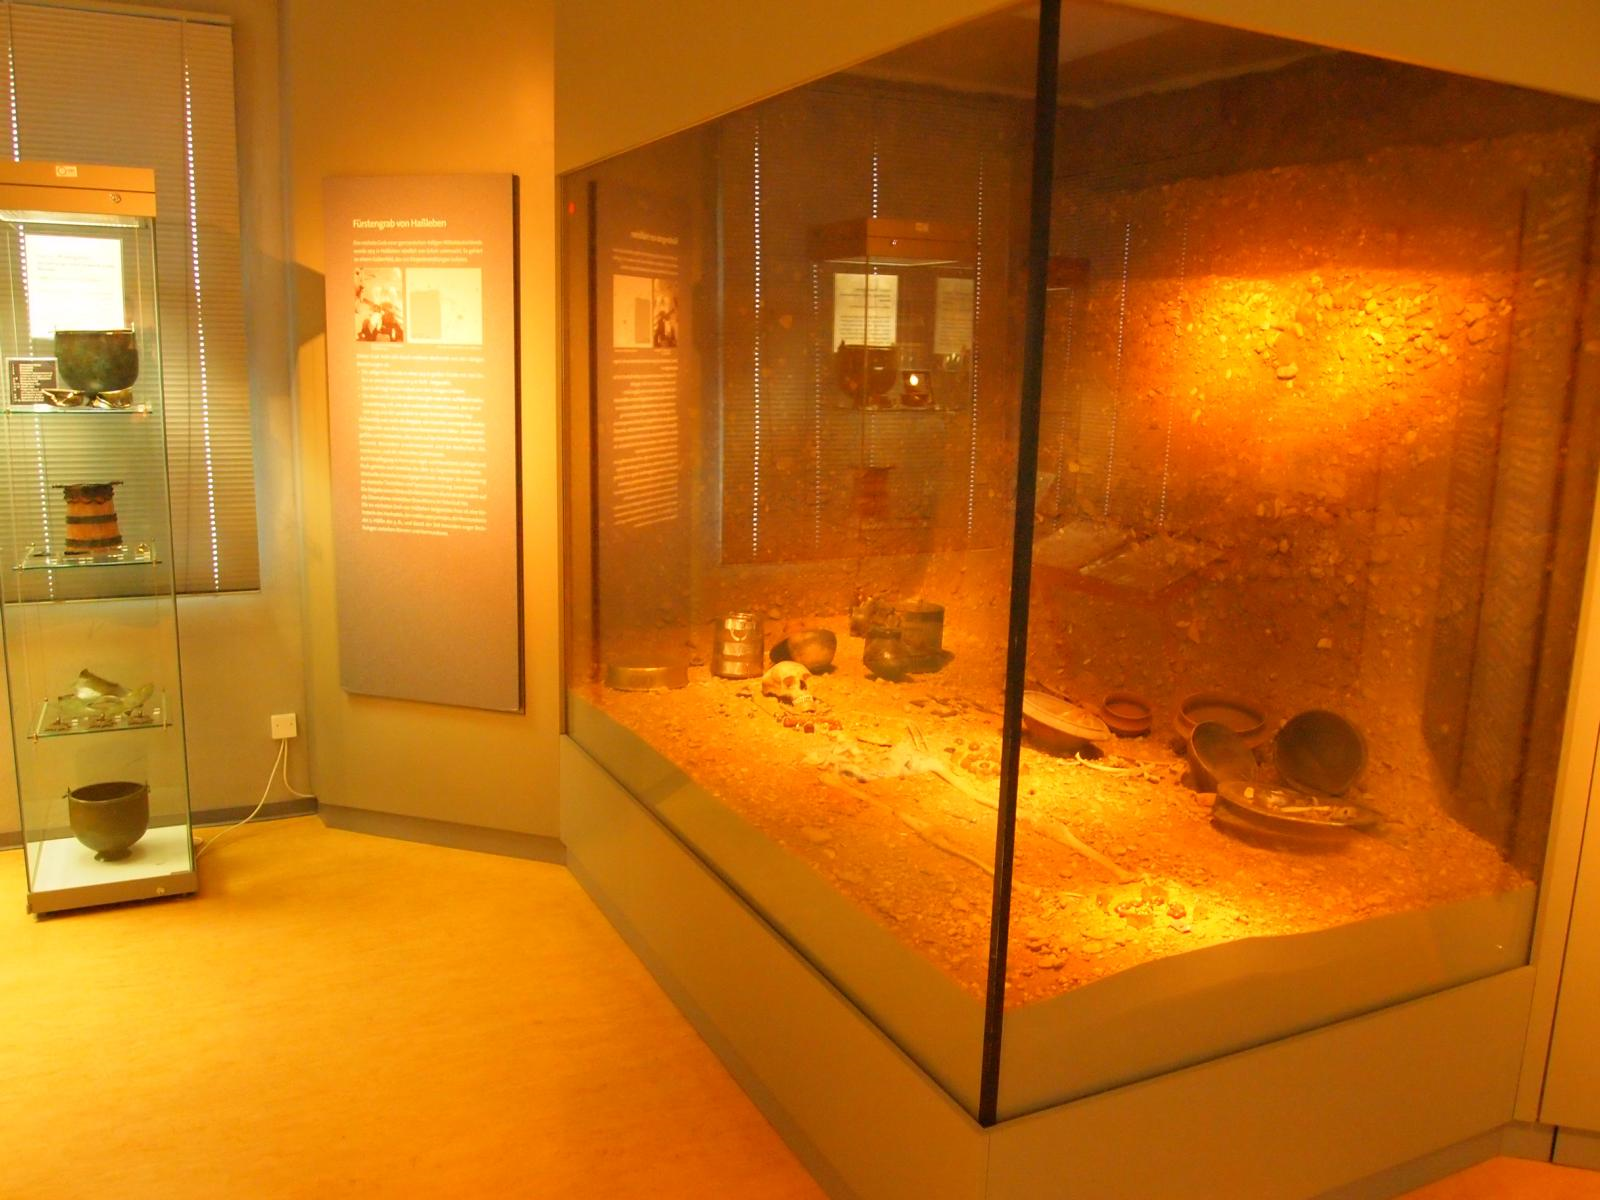
\includegraphics[width=0.8\textwidth]{../pics/Original.png}
	\caption{Original display of the Haßleben grave.}
	\label{fig:museums_original}
\end{figure}

After those field trips, I fashioned a presentation, in which I would introduce myself and previous projects I participated in. Later on in the meeting, I would show pictures of the museums in Limmerick and Vienna and explained the work, which had been done there. Finally, I prepared a short presentation of the Microsoft Gadgeteer-system and some of its capabilities. Following my presentation, the attending museum-staff, my professor end I discussed possible deployment scenarios. During the brainstorming the museum-officials named exhibits, which could or rather should receive more attention, whilst me and my professor suggested fitting solutions or explained further technological possibilities.
\\
At Pallais Schardt, the owners were very interested in technology, but they could not imagine how and where to make use of it. The best thing we could come up with was a guided tour. Thus, I was invited to one of their soirees with classical music and a tour of the house, in order to making up my own mind. Although it was very interesting, nothing ground-breaking arose.
\\
At Museum für Ur- und Frühgeschichte, the director was very fascinated by the demo and immediately came up with several exhibits, which seemed fitting to him. Yet, his optimism had to be reined a little. Some of the tasks he had in mind were unfortunately not realizable with the tools I had in hand.
\\
At Bienenmuseum, there were two main topics. First, social interaction of bees. For instance, bees dance to communicate the direction of plenty resources. Second, bees' perception of their environment. Bees see in another spectrum than we do and they can smell a lot better than us. In the end of our meeting, we were discussing about a virtual bee hive. This installation would be able
to simulate the behavior of a bee colony according to some certain inputs, which could be made by visitors.
\\
The final decisions were made after working out several key criteria for the best possible cooperation. Those were common criteria every museum could or could not meet and special criteria, which could also tip the scales. Three common criteria were identified. First of all, the amount and age of visitors was very important. Since the prototype had to be evaluated, a sufficient number of potential test subjects with a certain grade of affinity for technology would be needed. Second and not much less important, was the size and quality of the staff. If there was no expert of the museum's subject, who was able to work together with me, the project would be a fail. The third criteria was plainly budget. At some point, additional electronics and/or other equipment would be necessary. The special criteria more or less had an influence on the aforementioned main criteria. For example, monument protection, seasons, and motivation were some of them. First, Bienenmuseum had to go, because the club's chairman was not very fond of our discussions. Furthermore, the staff was not particularly professional and seemed to run the museum more as a hobby. The fact, that the museum has a large variety of visitors was a big plus, which was neutralized with the other fact, that bees are seasonal, and so are the according numbers of visitors. This makes an evaluation rather difficult, for not providing a constant number of test subjects.
\\
Finally, Pallais Schardt was struck from the list. Although, its owner was a restorer by trade, very approachable, and there were lots of events at the cafe, it had some corresponding cons as well. The building ant its historic role was very interesting, yet is a landmark. Thus, it must not be altered in any form, which might prove hard later on. The many people visiting the cafe are mostly 50 years an older. Hence, their abilities to understand and use technology as intended could be too much a risk during evaluation. Sadly, it is just a cafe and not a museum.
\\
The last item on the list is the Museum für Ur- und Frühgeschichte Thüringens. The major con was the planned exhibition, which leaves not much space for alterations. But, it is controlled by regional authorities. Hence, there is a budget for innovation projects. Moreover, the staff at the museum is interested in innovation and highly qualified in their field of expertise.

\chapter{Conception}
\label{conception}

After the \textit{Museum für Ur- und Frühgeschichte Thürigens} was chosen as a partner, all previous ideas had to be analyzed more thoroughly with feasibility in mind. Thus, impractical, and too complex or too simple ideas were eliminated in two rounds of review. At first, vague ideas were either improved or discarded. Hence, a screen displaying only information about a fossilized fireplace was eliminated. The idea of a system for digitizing stone carvings was considered too complex to realize and therefore discarded as well. Afterwards, some of the museum's staff and I looked at the contents, that could be provided for the remaining candidates. This left us with two remaining possibilities, that were promising enough from an educational as well as a technical standpoint. The first one was the reproduction of the \textit{Fürstengrab von Haßleben}, which contains replicas and original artifacts from a 1700 year old grave of a Teutonic princess. A close second was a workshop, which should have shown how archeologists and restorers work behind the scenes of a museum. Here, the latter consisted of too many single parts and a lot of questions remained unanswered.

%\begin{figure}[H] % [H] -> Here!
	%\centering
	%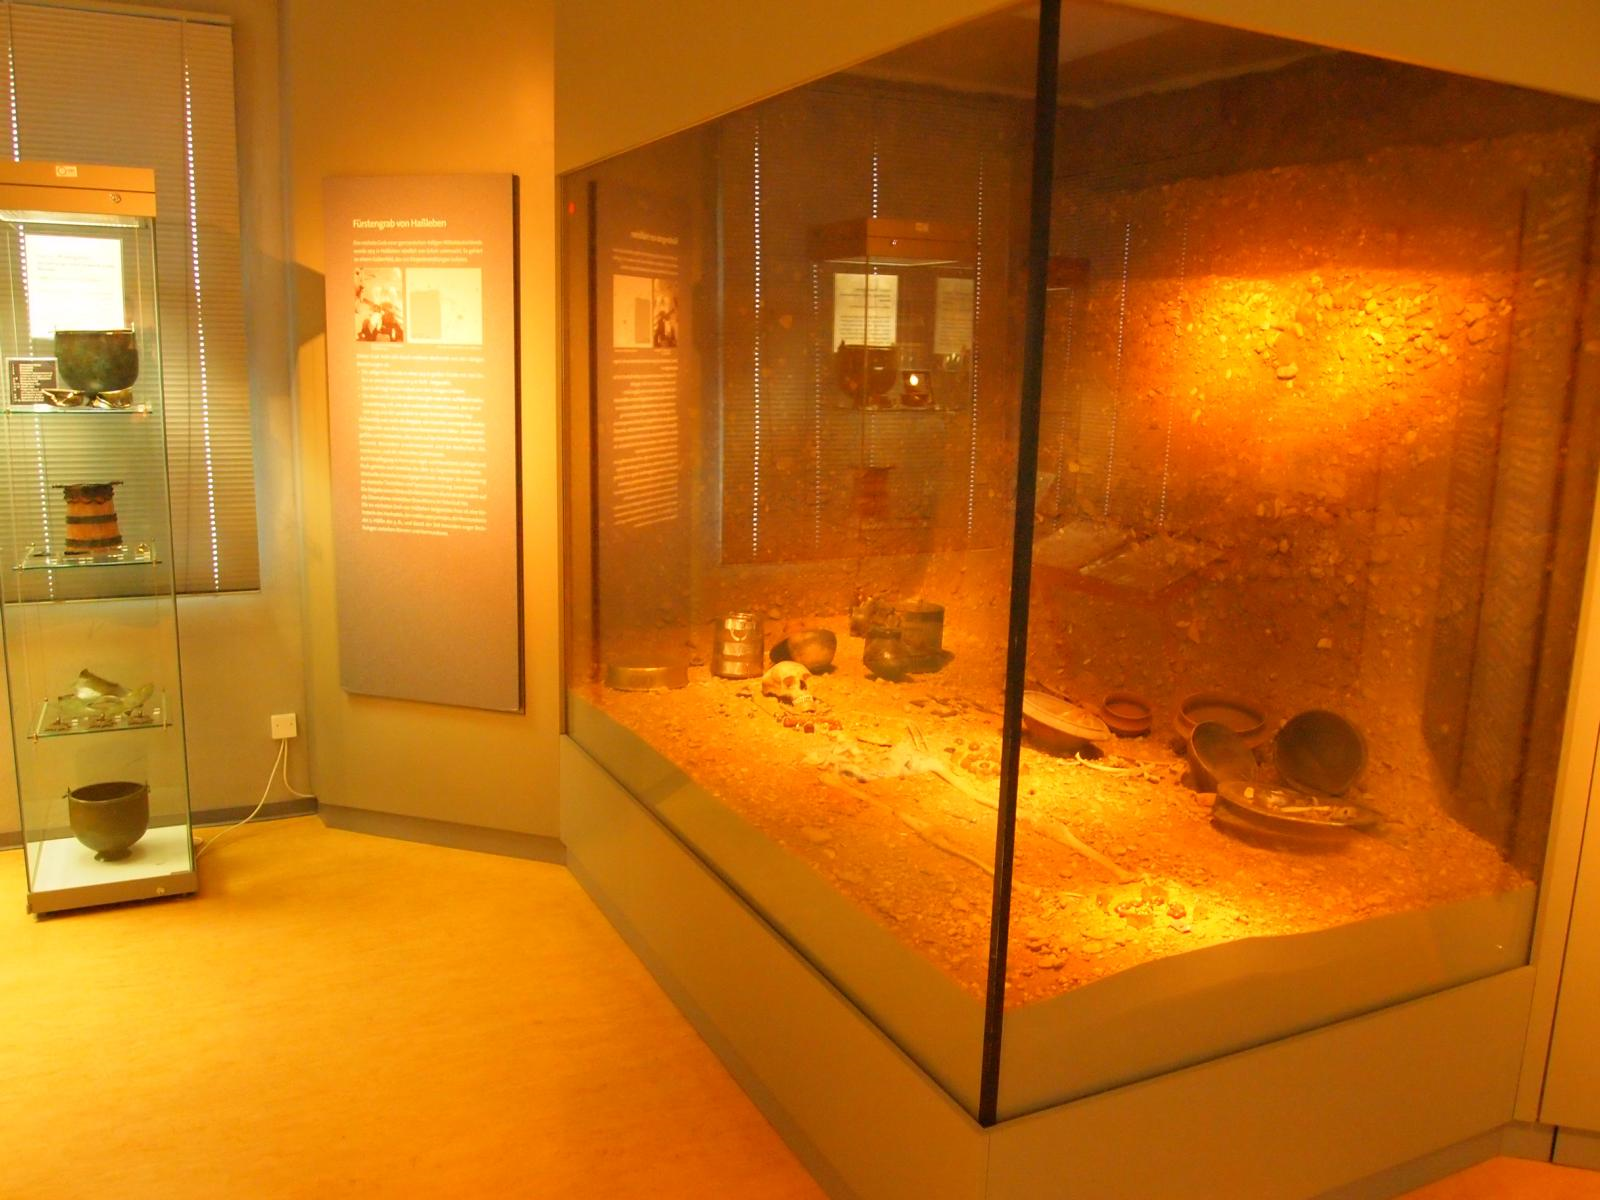
\includegraphics[scale = 0.7]{../pics/Original.eps}
	%\caption{Fürstengrab von Haßleben-showcase prior to installation.}
	%\label{fig:conception_grave}
%\end{figure}

According to the aforementioned review, the Fürstengrab von Haßleben was most promising and therefore chosen in the end. It contains many special relics from ordinary, Teutonic pottery to rare, Roman coins and jewelry. There are original artifacts and replicas on display inside the showcase, which I am collectively referring to as \textit{exhibits} throughout this work. Some of these exhibits are shown in Figure \ref{fig:conception_grave}a, b and c. The apparent eclecticism is, what makes the grave so special though. It is a sublime showcase for thriving trade and cultural exchange between Teutons and Romans as far east as Thuringia. Further, it proves how Teutons began adapting roman traditions, such as burials. In order to emphasize this insight, an interactive system was to be developed. Unfortunately, the showcase is located on the second floor. Thus, it does not get the attention it deserves. People are often tired after having visited the first floor. Hence, the museum's staff asked for an installation that would reactivate the visitors' attention.

%---------------------------------------------------------------------------- 

\section{System Preconditions}
\label{conception_system}

The system was to be developed and tested by me, and the museum-staff is responsible for its future maintenance. The full range of visitors' backgrounds cannot be foreseen. Some visitors might not have the proper technical experiences to operate contemporary interfaces. Consequently, it was crucial to design the system with that in mind. It had to be operable by absolute lay persons, who have no prior experience concerning information technologies. Hence, the interface had to be as intuitive and natural as possible. Four major points had to be considered.
\\
First, established and abstract input devices, such as keyboard and mouse, had to be replaced by something more natural. In order to be intuitive, the interaction was designed to capture and use the natural behavior of visitors. Outputs, on the other hand, had to be as discreet and as conservative as possible to not disturb or interfere with the exhibition. Thus, invasive technologies such as speakers and animatronics were excluded by the museum from the beginning. This consideration only left visual and haptic channels for output. The third point was, that daily operations at the museum were not to be compromised. So, it was not possible to develop the prototype inside the Haßleben-showcase itself and a full-size mockup had to be build somewhere else. Furthermore, the showcase and its precious exhibits had to be protected from any possible decay and nothing was to be rearranged. Thus, I measured the showcase and acquired a room in which a mockup could be placed for the prototype's implementation and testing\footnote{For a further description of the lab-setup see Chapter \ref{setup_development}}. Finally, the system's components, in- and output devices, had to be robust enough to cope with daily use. Moreover, they should also stay in their intended place. This meant that they had to be somehow attaching to the showcase.

In summary, the requirements for the final system were narrowing down the possibilities right from the beginning. Hence, we came up with several ideas and followed up on all of them, until one promised to be the most feasible.

%\paragraph{Annotations}
%
%\begin{itemize}
	%\item User perspective
	%\begin{itemize}
		%\item Visitor
		%\item Curator / staff
	%\end{itemize}
	%\item System view
	%\\
	%\item Development of ideas according to the plan
	%\begin{itemize}
		%\item Method of elimination
		%\item Feasibility
		%\begin{itemize}
			%\item Effort
			%\item Cost
		%\end{itemize}
	%\end{itemize}
%\end{itemize}

%-----------------------------------------------------------------------------

%\paragraph{Annotations}
%
%\begin{itemize}
	%\item Possibilities of hard- and software
	%\item Capabilities of a single programmer (me)
%\end{itemize}

%-----------------------------------------------------------------------------

\section{Concept Development}
\label{conception_constraints}

Developing the system, we followed two initial approaches. They were supposed to lead us to an intuitive, easy to use interface, which would be very naturally operable. The first concept featured the development of tangibles. Interactive objects would be placed outside the showcase and visitors would be able to interact with them. Haptic feedback would enable visitors to experience the exhibits in an unusual way. By touching replicas of otherwise locked up exhibits a deeper involvement is highly likely. Meanwhile, the other concept was based on gestural interaction. With this concept, visitors are enabled to interact with the showcase by pointing. This approach was based on the natural behavior of visitors. Like the previous approach an uncommon experience should raise visitors' involvement and attention.

\paragraph{Tangibles} 

The early idea behind this work was to work with \ac{MS} Gadgeteer to develop a tangible interface for and with a museum. Thus, we first thought about how to include those Gadgeteer-modules. Therefore, I built the demo device shown in Figure \ref{?}, which was based on a \textit{FEZ Spider Starter Kit}~\cite{SpiderKitGHI}. In addition, it utilized an \ac{RFID}-reader~\cite{RFIDreaderGHI} and a potentiometer~\cite{PotentiometerGHI}. The RFID-transponders were attached to an old 2,5" \ac{HDD} and a wireless mouse. When the \ac{RFID}-tags were recognized, an image of the object was displayed on the screen. By turning the potentiometer's knob the angle of view changed accordingly. This gave an impression of the possibilities of the hardware. Unfortunately, we only had two \ac{RFID}-tags that had the size of a credit card. After some research though, I found some tags for the correct frequency band and in sizes from a grain of rice over credit cards to key chains~\cite{RFIDtransponder}. Hence, including \ac{RFID}-tags in tangibles was feasible. 
\\
The shape and size of the tangibles were still up for debate. Another point was, whether the hardware would be placed inside or outside the tangibles. This decision dictates the shape and size of the tangibles and therefore the interaction. If it would be placed inside, the tangibles would have to be big. They would have turned out at approximately the size of a box of milk. Such an \textit{active tangible} would be handy and a whole system could be concentrated in one device. On the other hand, they would be prone to damage and maybe even theft. Hence, the tangibles would have to be tough and in some way attached to the showcase. In addition, batteries would have to be either charged or changed. This would take a certain amount of maintenance.
\\
With the hardware outside the tangibles and hidden in a pedestal in front of the showcase, the tangibles could be smaller. Moreover, \textit{passive tangibles} grant more flexibility concerning the shape as well. As described earlier (see Chapter \ref{motivation_interfaces} in ~\cite{TangibleUI}), the tangibles could have different features depending on certain properties. In this case, several \ac{RFID}-tags could be placed in each tangible. Depending to their \textit{constrained} collocation on the \ac{RFID}-reader, different reactions of the system could be triggered. In contrast to Ullmer at al., 2005, though, this affordance would be hidden and thus less obvious. The tangibles would have to be attached to the pedestal as well, although they would be less expensive to replace.

Both approaches had their advantages and disadvantages and none of them was concrete enough to make a decision. Thus, we continued to specify the concepts depending on their strengths and weaknesses. We did this, by anticipating probable relations between the exhibits inside showcase and the behavior of visitors behind the glass. There are several things visitors tend to do, if they are interested in an exhibit. They would like to inspect it up close. First, this means they would like to touch an exhibit and feel it. Second, they want to see it in more detail and from different angles. Next and induced by restrictions, visitors talk about an exhibit or  request further information. This could be anything from its age to where and how it was found.
\\
An active tangible could provide nearly all of those qualities in one package. It could - like the demo device - be fitted with a display and an \ac{RFID}-reader. The corresponding \ac{RFID}-tags could then be placed close to the device in order to trigger a particular output. Those outputs could be saved either on the device itself or provided by a server. The question of how to trigger different reactions was to be answered next. The device could either be placed on a pedestal equipped with \ac{RFID}-tags or the tags had to be brought to the reader in any other way. As mentioned earlier, an active tangible would be sizable and it would have to be related to the showcase's topic as well. Hence, it would be reasonable to combine those two criteria and fabricate enlarged reproductions of exhibits from the showcase. In order to fit the whole hardware, an active tangible would have to have a simple shape. This unfortunately excluded several of the more interesting exhibits, such as coins, a golden ring and other jewelry. Some options remained though. There was a skull, pottery and the metal remains of two jewelry boxes.
\\
The passive tangibles did not appear to cause this much consideration. Any exhibit could have been \ac{3D} scanned\footnote{The scans could have been done in the labs of the chair of Computer Vision and Engineering at Bauhaus-Universität Weimar.}, turned into a digital model, appropriately altered to fit an \ac{RFID}-tag and then printed or milled out. The printed or milled reproduction could be used as a positive to produce casting molds, afterwards. Thus, replacing damaged or otherwise lost tangibles would be more cost-efficient. In addition, it could be done by the museum-staff themselves. One or more \ac{RFID}-readers could be placed in a pedestal in front of the showcase. Depending on the \ac{RFID}-reader and a tangible's tag, the system would display the corresponding output.
\\
During those considerations, a third possibility came up. A hybrid approach that combined both principles was possible as well. The reproduction of a jewelry box could be turned into an active tangible and passive tangibles could be put inside to trigger an output. The \ac{RFID}-reader would be placed underneath the box's floor and the display in the lid. In order to provide different types of content, we thought about also producing two different types boxes. A more or less \textit{authentic reconstruction} made of wood and metal fittings could provide authentic information about a passive tangible's cultural background. Meanwhile, the other box could be constructed of transparent material, which would allow the user to see the hardware. This \textit{futuristic reconstruction} could provide statistical content for the same passive tangible.

However, the main problem remained with all approaches. Some kind of pedestal would have to be built and placed outside the showcase to hold the active and/or passive tangibles. Although passive tangibles would have been more cost-efficient to replace than active ones, maintenance was rated too high. Furthermore, if the pedestal was not to obscure the showcase, it would have been too low\footnote{The height of the showcase floor is about 65cm. For more details see Chapter \ref{installation}.} to grant satisfactory access for any visitor.

%-----------------------------------------------------------------------------

\paragraph{Pointing}

%As a result of the earlier drawbacks, we tried to minimize the objects outside the showcase. Hence, the display should be put inside.

The alternate concept took a completely different approach. It was more related to \ac{VR} and the interaction in \ac{3D} environments, where users are pointing at an object to select it~\cite{VRObjectSelectionCnG}. The underlying idea was to develop an information system that would be based on pointing-based interaction. A user points at an exhibit inside the showcase, the system recognizes the gesture, calculates the intended target and displays the corresponding information.
\\
Since the display should not interfere with the exhibits or occlude them, we had to make decisions about the position, size and type of the display. In order to not occlude exhibits, the display should not be placed in front or above the exhibits. Directly behind the glass panel would also have been problematical. It should have been placed along the visitors' viewing direction as they already would be looking into the showcase. This way, it would still imply coherence through visual proximity. A monitor on the one hand, and a projector on the other were two possible technologies to choose from. Both came with their own challenges. While a projector would have been easier to conceal than a monitor, a monitor would produce less heat and noise. Because most of the visitors approach the showcase from the long side and tend to stay there for most of the time, the display should be visible from this direction. This meant placing the projection plane or display on the opposing wall. Another solution for a projector came up during this consideration. A \ac{PDLC} switchable film~\cite{PDLC} could have been placed on the glass panel. Whenever the system was activated, the film and projector could have been activated as well\footnote{A \ac{PDLC} switchable film can be switched between a transparent and an opaque state. In its opaque state, it can be very well be used as a projection surface~\cite{PDLC}.}. Unfortunately, this solution would have been too expensive and difficult to install. A projection in the other direction was also disregarded, because the cost and heat issues caused by a projector were considered to high. Heat produced by a projector causes issues regarding the artifacts' conservation and is a safety risk for the sealed showcase. Therefore, we decided to install an LED-screen. It should be placed inside the showcase close to the exhibits.

\textit{Object selection in \ac{VR}-environments}~\cite{VRObjectSelectionCnG} and the \textit{SMSlingshot}~\cite{SMSlingshot}, nearly always use a \textit{pointing device} of some sort. With such a device, a potential user could directly point at the original exhibits within the showcase and trigger the corresponding reaction of the system - displaying related information. As described in detail in Chapter \ref{evaluation_pre}, I observed interactions between visitors and the showcase as well as between each other. During the pre-study, it turned out that visitors often pointed at the particular exhibits they were talking about. The interface could be designed to emulate this natural interaction between visitors and incorporate of the natural behavior.
\\
The first intention was to rebuild the SMSlingshot with Gadgeteer-hardware. The tangible was equipped with a microcontroller, a small display, a keyboard, a green laser, a wireless transmitter and of course batteries. A PC was used to put all the information together and render the output. Therefore, it had a camera to track the point a user was aiming at and a corresponding transmitter to receive the fired messages~\cite{SMSlingshot}. All those modules could be provided by Gadgeteer except the laser. A laser could have been controlled with a \textit{Breakout module}~\cite{BreakoutGHI} and a relay. However, shooting a laser into the showcase was a delicate issue. Hence, this solution had to be revisited, because for safety reasons it was not feasible. There could have been injuries of visitors' eyes or some of the precious exhibits might have reacted to the laser's energy in a corrosive way. We did not want to take those risks, but we were very keen on the idea of pointing interaction. Thus, I looked for other tracking methods. We could have used a tracking system similar to the aforementioned ones used in \ac{VR}. Those systems are expensive to install and maintain, though. Moreover, a proper compatibility with Gadgeteer was doubtful. So, I started looking for alternatives to Gadgeteer, too. Two established systems immediately came to mind. First, the \textit{Nintento Wii}, which uses a wireless device with pointing capabilities and additional inputs. Second, the \textit{\ac{MS} Kinect}, which is able to recognize free-hand gestures and might not require any device. Both are comparably inexpensive to acquire, have experienced support and communities and use less dangerous \ac{IR} light.
\\
The decision between the two was made according to the same criteria as mentioned above. Pointing with no device should be a more intuitive way to interact with the exhibition and other visitors than any handheld device. Furthermore, the restraint to use the system should be reduced. No tangible or pedestal would have to be created and attached to the showcase, which decreased cost for maintenance. Hence, the \ac{MS} Kinect was chosen.
\\
There is a Kinect for \ac{MS} Windows along with a special \ac{SDK} for \ac{MS} Visual Studio. As it turned out, the hardware inside the \ac{MS} Kinect was developed by \textit{PrimeSense} and is also used by the \textit{ASUS Xtion PRO}. This \ac{3D}-sensor is less expensive and smaller, which allows to be less intrusive inside the showcase. Besides, we already had some of them at the faculty, which meant that I could start developing right away. Another change was the decision for an open source \ac{SDK} called \textit{OpenNI}\footnote{OpenNI was co-founded by PrimeSense, a hardware developer that produces \ac{3D} sensing hardware. In November 2013 PrimeSense was bought by Apple, whereupon OpenNI was shut down.}, which in combination with its add-on \textit{NiTE} enabled me to use \textit{skeleton tracking}. This was critical for my approach, because I needed to have a \ac{3D} vector in order to be able to calculate where a user was pointing. Skeleton tracking would deliver the joints of a tracked person. Hence, I was able to retrieve the directions a limb is oriented in. If this vector was extended, I was able to calculate its possible intersection with an exhibit. More about used software and the exact calculations can be found in the next chapter.

The last topic that needed addressing was \textit{feedback}. Since there would be no haptic or acoustic feedback, and no \textit{glowing dot} produced by a laser either, future users would need another visual feedback in order to be able to see where they were pointing and determine how to correct that. Once more, Gadgeteer could have provided a solution. Our first idea was to replace the laser's dot by a spotlight. The system would calculate the position a user was pointing at and transmit it to a Gadgeteer-system. It would then move a special highlight to this position within the showcase. Only two actuators would be sufficient. The maintenance of this kind of installation could become very complicated though, because the system would have to be installed on the ceiling of the showcase. Actuators need to be calibrated regularly and mechanical gearing will wear out. Hence, this realization concept was dismissed. Nevertheless, the principle should remain the same. Thus, the aforementioned position would now be shown on an overview of the showcase on the display.

%\paragraph{Annotations}
%
%\begin{itemize}
	%\item Technical
	%\item From the museums perspective
	%\begin{itemize}
		%\item Size
		%\item Cost
		%\item Inclusion
	%\end{itemize}
	%\item Limitations of hard- and software
	%\item Capabilities of a single programmer (me)
%\end{itemize}

%-----------------------------------------------------------------------------

\section{Final Concept}
\label{conception_final}

%\textbf{Soll ich hier nochmal das Gesamtkonzept zusammenfassen oder ist es besser, das Organisatorische noch etwas mehr zu vertiefen und dafür das fertige System im Implementation-Kapitel genau zu erklären? -- Dann muss ich hier nochmal die Überschrift ändern.}

The final system consists of a \textit{depth sensor}, a \textit{PC} and a \textit{display}. All of the hardware is placed inside the showcase. In addition, an active tangible to remotely activate and deactivate the system should be developed as well. It was only intended to be a feasibility study, which determines if and how active Gadgeteer-tangibles might be incorporated into the system, later. Suitable components were recommended by me and provided by the museum after to mutual agreement.

The system requires two pieces of software. The first software is of an administrative nature and allows the museum staff to define and maintain the whole exhibition. The second software is presenting the exhibition to the visitors. Previously defined exhibits are selectable.
\\
The exhibition can be defined by museum-staff themselves. Therefore, an exhibition plane has to be defined and validated first. After that all the exhibits' positions on the plane can be defined and validated. Those positions can be defined in the same way users later interact with the system, by pointing. To exclude a certain inaccuracy when defining a position, it would have to be defined from different angles and validated afterwards. The whole process will be described in Chapter \ref{installation} and the technical execution in Chapter \ref{installation_tech}. Furthermore, the corresponding contents such as explanatory texts and detailed images are provided by the staff. Contents and positions can be changed, removed from or reloaded into the exhibition.
\\
When one or more visitors enter the area in front of the showcase the system recognizes them and reacts in an inviting fashion. A defined interaction space enables the user to interact with the system by pointing at an exhibit. No devices outside the showcase are needed. 

\paragraph{Functional Specification Document (\ac{FSD})} The final concept all parties agreed on was written down by me in an \ac{FSD} and responsibilities were covered by a contract. The document states, which features of the final system must, should and must not be implemented and working.
\\
The necessary features or \textit{must-criteria} where that the the system would have to have separate modes for administration and presentation of an exhibition. The visual feedback of the interaction would be provided by the display. Visitors would be automatically recognized by the system, but only one user at a time would be able interact with it. The whole system would be maintainable by the museum's staff and will start and shut down automatically.
\\
Preferable features \textit{should} be realized, but would not be mandatory. Thus, there should be a system's manual. For guided tours, it should be further possible to switch the system into a 'blind' mode, where it does not react to people. Extensive exhibits should have a slide show. The system should be operable with either the left or right hand. In addition, statistics about the system's use should be logged for later analysis.
\\
There were also criteria that were not requested, and therefore \textit{must not} be implemented. Any free-hand gestures other than pointing must not be recognized by the system. Further, the lighting inside the showcase must not be controlled or influenced by the installation. Feedback has to be only visual and not auditive or haptic. Hence, speakers or tangibles must not come to use. 
\\
Furthermore, the \ac{FSD} describes system requirements concerning hard- and firmwares, data formats and other organizational parameters. 

In addition to the \ac{FSD}, a contract was drawn up by the university's layer's office. It sorted responsibilities and was later signed by the museum's director, my professor and me. Both documents can be found in the appendix.

%\paragraph{Annotations}
%
%\begin{itemize}
	%\item 'Pflichtenheft'-criteria
	%\begin{itemize}
		%\item Must
		%\begin{itemize}
			%\item 
		%\end{itemize}
		%\item Should
		%\begin{itemize}
			%\item 
		%\end{itemize}
		%\item Could
		%\begin{itemize}
			%\item 
		%\end{itemize}
		%\item See appendix
	%\end{itemize}
	%\item Contract 
		%\begin{itemize}
			%\item MUFT, BUW and me
			%\item Avoid misconceptions
			%\item Commitments / Obligations
			%\item Responsibilities
			%\item Boundaries
			%\item Legal stuff
			%\item See appendix
		%\end{itemize}
%\end{itemize}

\chapter{Setups and Hardware}
\label{installation}

Three installations were build. One lab-setup for development, one makeshift setup was placed in the faculties lobby, and the final one was installed inside the showcase in Museum für Ur- und Frühgeschichte Thüringens. The various setups differed more or less in dimensions and were run with different hardwares. Early tests were conducted with the lab-setup. The lobby-setup was used for a stress-test during an open door-event at the faculty, whereas the final evaluation took place in the museum. Then, only the presentation-software was tested.

%\paragraph{Annotations}
%
%\begin{itemize}
	%\item Current State
	%\begin{itemize}
		%\item Comparing Lab- and Summaery-setup
		%\item Documentation of system's installation
	%\end{itemize}
%\end{itemize}

%-----------------------------------------------------------------------------

\section{Lab-setup}
\label{installation_lab}

A special lab had to be found and equipped with all necessary Hardware. The Hardware was lend to me by multiple sources of the faculty, while the museum's carpenter made a pedestal consisting of a surface and feet. The surface is made out of four 9mm-press boards. The feet seemed to unstable and thus were replaced with one desk rack for each board.

%-----------------------------------------------------------------------------

\section{Lobby-setup}
\label{installation_lobby}

After some technical difficulties with the museum-setup, the first test under aggravated conditions was conducted during \textit{Summ\ae{}ry}\footnote{Summ\ae{}ry is an open door-event at the faculty of media, where all chairs present their work throughout the faculty-buildings.}. Therefore, I build a makeshift setup in the facultie's lobby. It consisted of three tables forming the exhibition plane and a bar table, on which the computer and a tripod with the sensor on top were positioned. There were three targets - a candy bar, a stack of coins, and a stack of fliers - lying on the plane (\textit{see Figure}).
\\

%-----------------------------------------------------------------------------

\section{Final museum-setup}
\label{installation_museum}

\begin{itemize}
	\item Automatic boot at 8:30am [Bios]
	\item Runnging
	\item Logfiles for each \textit{Session-Event}
	\begin{itemize}
		\item Start Session: User in interaction zone (Exhibition.UserPosition +/- Threshold from SessionHandler := 250mm)
		\item New Target: User pointing at a target
		\item Target Selected: Dwelltime (Exhibition.SelectionTime := 700ms) starts slide show for selected target
		\item End Session: User leaves interaction zone
	\end{itemize}
	\item Automatic shutdown at 4:45pm [Software]
\end{itemize}
\chapter{Implementation -- Interactive Museum Installation}
\label{implementation}

The \ac{IMI}-system consists of two main parts. First, the hardware, which involves the physical tracking and computing of that data in the background. Second, the software, which includes the \ac{IMI}-libraries and pieces of software utilizing them.

%\paragraph{Annotations}
%
%\begin{itemize}
	%\item Explanation of functionalities
	%\item Diagrams
	%\begin{itemize}
		%\item Classes
		%\item Sequences
	%\end{itemize}
	%\item Sketches
%\end{itemize}

%-----------------------------------------------------------------------------

The hardware consists of and PC, the sensor, a screen and peripheral input devices for maintenance. The designated PC is an \textit{ASUS VIVO VC60-B013M}. It employs a \textit{Intel Core i5 3210M} with a clock speed of 2x2,5GHz and 4GB DDR3 SDRAM~\cite{VivoPCVC60}. Since the system does not have complex graphics, there was no need for a sophisticated graphics card. Hence, the PC is compact and does not need much electricity. 
\\
As a display, we chose an \textit{ASUS MB168B+} with a size of 15.6'' and es resolution of 1920x1080 pixels. The display further houses its own graphics chip, which enables it to be connected to a PC via a USB3.0-cable~\cite{MB168B}. This configuration eased the installation, because of the smaller plug the holes drilled into the back wall of the showcase could be smaller than for a usual display-cable. The display is supported by a modified bookend, which is attached to the back wall with two screws. An additional hole has been drilled for the cable. This hole is hidden by the display. Although it was planned to camouflage the display with a foil, it did not seem necessary, because lighting at the new position of the display is already dim.

The soft- and firmware used for developing and running the system is based on \textit{\ac{MS} Windows 7 Professional x86}. As mentioned earlier, the software was included into \ac{FUBI}. This framework is available as an \textit{\ac{MS} Visual Studio 2010}-project. The all software is written in \text{$C\#$} and hence makes use of the \textit{\ac{MS} .NET Framework 4.5.1}~\cite{MSNET} and further \textit{\ac{MS} XNA Framework 4.0}~\cite{MSXNA} for certain functions throughout certain regions of the software. Moreover, \ac{FUBI} utilizes the functionalities of \textit{OpenNI 2.2.0.33}~\cite{OpenNI} and \textit{NiTE 2.2.0.11}~\cite{NiTE}. 

%------------------------------------------------------------------------------

\section{Libraries}
\label{implementation_libraries}

\ac{IMI} includes a collection of libraries, which can be used to implement interactive applications. At the time the functionality is restricted to free-hand pointing gestures. Other mechanisms can be easily added. An \ac{IMI}-exhibition is modularly build by those libraries. The Exhibition- and Exhibit-class have structural functionality and manage an exhibition's data. Meanwhile, the Handler-classes use this data to generate and operate the interaction between user and system.

\paragraph{Preliminaries} Terms used hereafter are depicted by Figure \ref{implementation_terms} and defined as follows:
\begin{itemize}
	\item A point or corner is a point in \ac{3D} space of type \texttt{Point3D}.
	\item A plane is defined by three points or corners. 
	\item A position is a point on a plane of type \texttt{Point3D}.
	\item A kernel is an exhibit's membership function. It has a size and radius.
	\item A target is an exhibit's representation on the exhibition plane. It is determined by its position and kernel.
\end{itemize}

\textbf{F I G U R E}
%\begin{figure}%
%\includegraphics[width=\columnwidth]{filename}%
%\caption{.}%
%\label{fig:implementation_terms} %
%\end{figure}

%-----------------------------------------------------------------------------

%\paragraph{Annotations}
%
%\begin{itemize}
	%\item 'What are the libraries?'
	%\begin{itemize}
		%\item Overview
		%\item Structure of Exhibition and Exhibits
	%\end{itemize}
	%\item 'What does each one do?'
	%\begin{itemize}
		%\item Modularity
		%\item Config-files (XML)
		%\item Particular methods (Lotfußpunkte, Ebenenschnittpunkt, DataLogger etc.)
	%\end{itemize}
%\end{itemize}

\paragraph{Exhibition.cs} Members of the Exhibition-class are needed to define an \ac{IMI}-exhibition. All necessary information is contained and managed in this class.

The \texttt{exhibitionPlane} is the most essential component of an \ac{IMI}-exhibition. All exhibits' positions are defined on this fundamental property. It is constructed by three corners. The structure of such a Plane is declared by the GeometryHandler-class. The Exhibition-class further holds a list of \texttt{Exhibit}-objects. In this \texttt{List} all selectable \ac{IMI}-exhibits of an \ac{IMI}-exhibition are stored. In addition, the earlier mentioned user position that defines the interaction space is also saved in this class as a point. An \ac{IMI}-exhibition's name and file path are members of the Exhibition-class, too. So are the images, which are used to camouflage the display against the background and the overview of the exhibition plane with sketches of exhibits in their respective positions. Furthermore, data crucial for interaction are also members of this class. So are the default values for the threshold needed for defining exhibits and the dwell time for target selection. Timespans used by the presentation software are \texttt{lockTime}, which determines a short period of paused interaction after selecting a target and \texttt{slideTime} which determines for how long a single image is shown during an \ac{IMI}-exhibit's presentation.

The characteristic functionality of the Exhibition-class is its get- and set-methods. They allow for reading and writing all those essential variables.

%------------------------------------------------------------------------------

\paragraph{Exhibit.cs} The virtual representation of an \ac{IMI}-exhibit is structured by the Exhibit-class. This includes data relevant for interaction with the system and an \ac{IMI}-exhibit's presentation upon selection. Like an Exhibition-object, an Exhibit-object stores its own file path as well. This is necessary for organizational reasons. 

The most important member of an \ac{IMI}-exhibit is its position. In combination with the two kernel-defining members \texttt{kernelSize} and \texttt{kernelRadius} the SessionHandler-class is able to compute which target a user is pointing at.  

Members relevant for the presentation of an \ac{IMI}-exhibit are its name, descriptive text and collection of images. The images are stored in a \texttt{Dictionary} as a pair of an image's file path and the image itself. 

The Exhibit-class, just like the Exhibition-class, is of structural nature and therefore only has the same administrative methods that get and set members.

%------------------------------------------------------------------------------

\paragraph{FileHandler.cs} The objective of the FileHandler-class is \textit{saving} and \textit{loading} data of an \ac{IMI}-exhibition, its exhibits, and all their properties. Therefore, a temporary Exhibition- and Exhibit-object are needed. Exhibitions along with all related information are saved in \textit{XML-format}. The hierarchical structure of XML-files allows adding, changing and removing elements without much effort. 

To save an \ac{IMI}-exhibition and all its properties several XML-files have to be written. The main file contains the aforementioned defining properties of the exhibition. This means that each \ac{IMI}-exhibit is stored separately. It is saved as an XML-file as well. Each \ac{IMI}-file contains all properties as attributes or \textit{forwarding file paths}. Equally, corresponding images are saved as file paths leading to the actual image. The exhibition plane is also separately saved as an XML-file. 
\\
Loading works in reverse to this procedure. As en \ac{IMI}-exhibition is being loaded, its properties are either saved into a \textit{temporary Exhibition-instance} or forwarding file paths are followed. A \textit{Temporary Exhibit-instance} is used to load all of an \ac{IMI}-exhibits.
\\
The modular composition allows the \ac{IMI}-system to be flexible. \ac{IMI}-exhibits exist as independent entities and can be easily removed from or added to an existing \ac{IMI}-exhibition. The same applies for the exhibition plane. Figure \ref{fig:filehandler_data_structure} depicts the whole data-structure behind an \ac{IMI}-exhibition.

\textbf{F I G U R E}
%\begin{figure}%
%\includegraphics[width=\columnwidth]{filename}%
%\caption{.}%
%\label{fig:filehandler_data_structure} %Entity-Relationship
%\end{figure}

An additional function of the FileHandler-class is reading TXT-files. This feature is used to load pre-written descriptions of \ac{IMI}-exhibits.

%------------------------------------------------------------------------------

\paragraph{GeometryHandler.cs} The GeometryHandler-class is solving essential computations of analytic geometry-problems. Therefore, the two structs \texttt{Vector} and \texttt{Plane} are declared, because standard types of C$\#$ do not deliver the complexity needed for those computations.
\\
A \texttt{Vector}, in contrast to a standard \texttt{Vector3D} or \texttt{Vector3}, is not only a \textit{direction vector}. It also has a \textit{starting} and a \textit{terminal point}. Hence, a \texttt{Vector} $V_{IMI}$ is defined by a starting point $P_{S}$ and either an endpoint $P_{E}$ or a direction vector leading towards it $\overrightarrow{d_{E}}$, where $P_{S}$ is either a user's tracked head- or elbow-joint and $P_{E}$ is its tracked hand-joint. 
\begin{align*}
	V_{IMI} &= P_{S} + \overrightarrow{d_{E}} \\
	V_{P} &= P_{S} + \lambda_{P} \cdot \overrightarrow{d_{E}}
\end{align*}
As the factor $\lambda$ is varied, any point $P$ along a \texttt{Vector}'s direction of propagation can be expressed. 
\\
A \texttt{Plane} is defined by one starting corner $C_{1}$ and either two additional corners $C_{2}$ and $C_{3}$ or two additional \texttt{Vector}s $\overrightarrow{d_{C_{2}}}$ and $\overrightarrow{d_{C_{3}}}$ towards those corners. In short, a \texttt{Plane} $E_{IMI}$ is defined by two \texttt{Vector}s $V_{C_{2}}$ and $V_{C_{3}}$ of identical origin.  
\begin{align*}
	E_{IMI} &= V_{C_{2}} + V_{C_{3}} \\
	E_{IMI} &= C_{1} + \lambda_{C_{2}} \cdot \overrightarrow{d_{C_{2}}} + \lambda_{C_{3}} \cdot \overrightarrow{d_{C_{3}}} \\
	E_{P} &= C_{1} + \lambda_{P} \cdot \overrightarrow{d_{C_{2}}} + \lambda_{P} \cdot \overrightarrow{d_{C_{3}}}
\end{align*}
Any position $P$ on a \texttt{Plain} can be expressed by varying $\lambda_{C_{2}}$ and $\lambda_{C_{3}}$.

input-members: pointing- and aiming-points/positions
\\
calculation-members: classifications and combined Points/Positions

CHARACTERISTIC FUNCTIONS AND METHODS: 
\\- pointing- and aiming positions yield intersetions (pedal point and vector-plane) 
\\- FORMULA: pedal point
\\- FORMULA: plane-intersection
\\- classification and weighing

%------------------------------------------------------------------------------

\paragraph{CalibrationHandler.cs} Defines and validates Points, Positions and Planes
\\
samples per position and threshold

CHARACTERISTIC FUNCTIONS AND METHODS: 

%------------------------------------------------------------------------------

\paragraph{SessionHandler.cs} Determines the user from visitors. Further builds lookup-table and checks for intersections. Calculates the feedback of current pointing position and its buffering. Calculation of fbP on canvas.
\\
userPosition + radius $\Rightarrow$ ID
\\
lookup
\\
feedbackPositionBuffer and feedbackPositionBufferSize
\\
Intersections with ePlane: XNA-varialbles
\\
ScreenCoords: screenSize, canvasSize, planeCanvasRatio

CHARACTERISTIC FUNCTIONS AND METHODS: 

%------------------------------------------------------------------------------

\paragraph{StatisticsHandler.cs} Instant statistics such as average, SD usw. 

CHARACTERISTIC FUNCTIONS AND METHODS: 

%------------------------------------------------------------------------------

\paragraph{DataLogger.cs} Logs events during a session.
\\
path to save to
\\
paragraphs
\\
startSession (Timestamp)

CHARACTERISTIC FUNCTIONS AND METHODS: 

%------------------------------------------------------------------------------

\section{Administration-software}
\label{implementation_administration}

\paragraph{Annotations}

\begin{itemize}
	\item 'What is the administration-software?'
	\begin{itemize}
		\item Define and edit exhibitions
		\begin{itemize}
			\item ExhibitionPlane
			\item Define, load and remove Exhibits
			\item Define and change UserPosition
			\item Edit dwelltimes
			\item Load Background(s)
		\end{itemize}
		\item Define and edit exhibits
		\begin{itemize}
			\item Define and change Position
			\item Load and remove Images
			\item Write and load Description (up to 310 charcters)
		\end{itemize}
	\end{itemize}
	\item 'What does it do?'
	\begin{itemize}
		\item \textit{Sequences}
		\item Paper-mockup
		\item Create (re-)loadable Config-files
	\end{itemize}
\end{itemize}



\section{Presentation-software}
\label{implementation_presentation}

\paragraph{Annotations}

\begin{itemize}
	\item 'What is the presentation-software?'
	\begin{itemize}
		\item Display information of previously defined interactive exhibits
		\item Overview-map of ExhibitionPlane
		\item Feedback of exhibits' positions and pointing position
		\item Description (Readability, Sehwinkel) and Images as slide show
	\end{itemize}
	\item 'What does it do?'
	\begin{itemize}
		\item Check for Exhibition
		\item Pre-calculate Lookup for exhibit-selection (saves processing power)
		\item Recognize visitors
		\item Identify user by predefined UserPosition 
	\end{itemize}
\end{itemize}



\section{Presentation-remote}
\label{implementation_remote}

\paragraph{Annotations}

\begin{itemize}
	\item 'What is the presentation-remote?'
	\begin{itemize}
		\item Microsoft Gadgeteer-Device
		\item Bluetooth / WiFi-connection to PC
		\item For lecturers in order to explain exhibits themselves
	\end{itemize}
	\item 'What does it do?'
	\begin{itemize}
		\item Automatically connect to Presentation-software
		\item Toggle Presentation-software's blindness
	\end{itemize}
\end{itemize}



\section{Statistics-tool}
\label{implementation_tool}

\paragraph{Annotations}

\begin{itemize}
	\item 'What is the statistics-tool and what does it do?'
	\begin{itemize}
		\item Small tool to evaluate logged user-data
		\item Statistics, such as average length of stay/session, exhibits chosen and how many transitions 
	\end{itemize}
\end{itemize}

\chapter{Evaluation}
\label{evaluation}

The \ac{IMI}-system in its final configuration was developed to be a reliable for every day use and easy to maintain. Although tests in the controlled environment of the lab were promising, it had to proof itself in a realistic scenario. Therefore, the \ac{IMI}-system was installed inside the Haßleben-showcase. Afterwards, the \ac{IMI}-exhibition about the showcase was defined by the museum staff and me. The staff was responsible for descriptive texts, detailed images and the overview sketch for proper feedback. Meanwhile, I assisted during the definition of the exhibition plane and the exhibits' positions.

However, in order to determine, whether or not the \ac{IMI}-system raised awareness for the showcase's topic a pre-study had to be made. Therefore, the behavior of visitors around the un-augmented showcase had to be observed. In addition, their awareness of the showcase's contents had to be found out as well.

A true insight could only be gained by examining how the \ac{IMI}-system would be accepted by visitors over a longer period of time. Furthermore, they should not be influenced by as less unusual circumstances as possible.

%-----------------------------------------------------------------------------

\section{Pre-Study}
\label{evaluation_pre}

The Haßleben-showcase is at the beginning of the second room on the second floor of the museum. Visitors frontally approach it when the come through the door. There are several related showcases in the room. Among them is a coffin in the middle of the room. In the following room, a the topic changes. There is a pottery oven in the corner and a bench on front of it. From this bench, I observed visitors in the previous room with the Haßleben-showcase in it. To disguise myself, I had one of the museum's audio guides\footnote{The Museum für Ur- und Frühgeschichte Thüringens offers audio guides for free. Visitors only have to leave a deposit. The audio guide is an app installed on an iPod Touch. It provides brief information about certain showcases and exhibits. They are identified by a sticker with the number of the corresponding audio track on it. The audio guide has German and English versions of each track.} with me.  

The interaction of visitors with the showcase itself and amongst each other was observed and noted. Further, I noted the size of a group of visitors along with their age, which in some cases had to be estimated. When visitors left the \textit{Haßleben-room}, they were asked about the showcase. The intention was to gain information about their grade of awareness considering the Haßleben-showcase. Therefore, I conducted a \textit{semi-structured interview} with each group of visitors leaving the Haßleben-room. 
\\
I hypothesized that the awareness considering a showcase can be graded into the following three stages:
\begin{enumerate}
	\item Awareness of its \textbf{mere existence}.
	\item Awareness of its \textbf{general composition}.
	\item Awareness of its \textbf{specific composition}.
\end{enumerate}  
Hence, my questions were intended to grade each group of visitors with respect to those stages. In the end of the interview visitors were asked about their visiting habits concerning museum. The questions were:
\begin{itemize}
	\item 
	\item 
	\item 
	\item 
	\item 
	\item 
	\item 
\end{itemize}
All observations and answers were noted in a protocol-sheet, which can be seen whole in the Appendix of this work. 

This lead to data that was of a qualitative nature. Whereas quantitative data can be statistically analyzed, qualitative data has to be handled in a different fashion.

Ergebnis

%-----------------------------------------------------------------------------

\section{Study}
\label{evaluation_study}

\paragraph{Annotations}

\begin{itemize}
	\item Pre- and postcondition of exhibition
	\item Survey of visitors' behavior prior to system's installation and afterwards
	\begin{itemize}
		\item Interaction between visitors
		\item Interaction with display
		\item \ac{LOS}
		\item Interviews
		\item Evaluation-Forms
	\end{itemize}
\end{itemize}

Bimodale Verteilung der 1. Stichprobe gegen modale Verteilung der 2. Stichprobe

%-----------------------------------------------------------------------------

\section{Post-Study}
\label{evaluation_post}

\chapter{Discussion}
\label{discussion}

The pre- and main study were conducted during a period of five days. They both compare the awareness of visitors concerning the Haßleben-showcase and its exhibits. Therefore, visitors were observed during their time around the showcase and interviewed afterwards. The questions aimed at the participants \textit{stages of awareness} introduced in the previous Chapter.
\\
Moreover, a post-study was evaluated to gain an idea of how the \ac{IMI}-system was used by visitors when they did not feel monitored. Furthermore, the stored data can give an insight into necessary improvements of the current \ac{IMI}-exhibition of the Haßleben-showcase.

\paragraph{Samples and Comparability} During the pre-study 53 visitors participated in the interviews. They were distributed over 19 groups. That is an average group size of about 2.8 visitors per group. Their average age was 24.33 years. The properties of average age and group size of pre-study and main study are approximately the same. In the main study, 58 participants from 32 groups were participating. The average group size of 1.8 was considerable lower. However, the age was nearly identical. The average age of participants from the main study was 25 and hence only 6 months above the value of the pre-study.
\\
Nevertheless, the studies can not be treated as a between-subjects test. Reason for this restriction is the distribution of the participants' ages. Both samples do have the same average age, yet the distribution of the ages varies. While the sample of the main study is mostly normally distributed, the sample of the pre-study is not. Here, the distribution is trimodal. This means that both might have a similar average age, but the reason for this fact is different. Hence, the samples are not statistically comparable when it comes to that particular criteria. The distributions of the pre-study and main study can be seen in Figure \ref{fig:discussion_age-distribution}.
\begin{figure}[H]%
\includegraphics[width=\columnwidth]{../pics/both-age.eps}%
\caption{Age distribution of participants from the pre- and main study.}
\label{fig:discussion_age-distribution} 
\end{figure}

The majority of all casual visitors and invited participants of both studies were on an identical level of knowledge about the Haßleben-showcase. Thus, their engagement with the \ac{IMI}-system can be seen as impartial. There were sufficiently less casual visitors among the sample of the main study and, therefore, more technical experienced participants. Those pre-recruited participants might have been less restrained in using novel technologies. Their technical expertise, however, was of little use, because no devices had to be operated and the \ac{GUI} of the presentation software had not been shown to anyone prior to the main study. Hence, all participants, casual and invited, had to rely on their physical capabilities alone. Furthermore, only a few had prior knowledge of the contents of the \ac{IMI}-exhibition inside the Haßleben-showcase. Consequently, the answers of both samples can be seen as equally impartial, while the interaction of several pre-recruited participants is certainly more experienced.

%-----------------------------------------------------------------------------

\paragraph{Observed Interactions}

The first value that was observed about groups around the Haßleben-showcase was the \ac{LOS}, the duration visitors and participants were addressing the showcase. The average time visitors from the pre-study spent with the showcase was around one minute. The longest stay that was observed did not last longer than two minutes, while the shortest was between 0 and 30 seconds long. The shorted session during the main study was 48 seconds and the longest session took 13:11 minutes. On average the \ac{LOS} was 5:25 minutes. However, the pre-recruited participants were present to evaluate the presentation software and, therefore, stayed longer and were more engaged with the \ac{IMI}-system. Hence, the average and maximum \ac{LOS} of this sample is so much longer. Nevertheless, the post-study was conducted under daily circumstances and it revealed that the average \ac{LOS} was 1:34 minutes. This means an increase of the average \ac{LOS} of about 50$\%$. The difference between the longest (11:43 minutes) and shortest (11 seconds) stay was similar to that of the main study, whereas the observations from the pre-study only showed a small range of only two minutes. Thus, the shortest stay could not be improved by much, but the longest stay was nearly increased sixfold.
\\
In conclusion to these observations, visitors spent significantly more time with the Haßleben-showcase than before. Hence, the visitors are more engaged with the Haßleben-showcase. This should raise their awareness of its existence, as stated in Chapter \ref{evaluation}.

During the pre-study visitors perceived the Haßleben-showcase like any other showcase of the museum. They approached it and looked at the exhibits inside the showcase. Visitors did that from the broad and narrow side, whereas the narrow side was used four times less than the broad side. Seven groups out of 19 read the explanatory text. One visitor seemed to think about something and tried to look it up in the text. Some visitors went past the showcase or only glanced at its contents. The main study introduced the \ac{IMI}-system to the showcase and all visitors and participants were looking into the grave. The display drew their interest and they started interacting with the \ac{IMI}-system. Nearly every participant gave it a try and started pointing. Thereby, some issues arose. The main observation was that half of the 32 groups were over-fixated on the visual feedback given by the navigational view of the presentation software. Thus, they did not use the feedback to fine tune their pointing, but completely relied on it. Because the display was raised and not in their direct view on the exhibition plane, the feedback positions of the users began to tremble. The movement of their head to look up had changed their aiming position and consequently the feedback position as well. Additionally, some participants perceived the interface to be more natural than it was, and pointed with their left arm or tried other gestures such as a swiping move to change the images during the presentation of an \ac{IMI}-exhibit. Another fact that could be observed was that the readability was compromised by two factors. The letters or the display were too small and previously calculated time for reading was too short.
\\
Interaction of visitors during the post-study was not observable. Nevertheless, the amount of active sessions shows that the \ac{IMI}-system is used on a day to day bases by the normal audience of the museum. The quote of about 1:1 between active and empty sessions, however, does not have to necessarily mean that only 50$\%$ of all visitors take notice of the exhibits inside the Haßleben-showcase. If the durations of empty sessions would be evaluated as well, they will show for how long non-interacting visitors stay around the showcase. There \ac{LOS} might also be longer than before.
\\
Conclusively, it can be said that the presence of the \ac{IMI}-system has increased the engagement of visitors with the Haßleben-showcase and the \ac{IMI}-exhibits inside it. There are indicators for issues that need to be addressed to improve the interaction of visitors with the presentation software. 

After the augmentation of the Haßleben-showcase with the \ac{IMI}-system, visitors were more engaged with the exhibition. This involvement also influenced the interaction between visitors. Thus, their behavior among each other changed as well. During the pre-study, visitors moved in closed groups, clustered in particular places or walked through the museum floor individually. 31 out of the 51 visitors that were observed moved as a closed group. That is about 60.8$\%$ of all visitors. 25.5$\%$ moved individually and clustered in particular places and the remaining 5.7$\%$ (seven visitors) were moving detached from their group. In the main study only two cases of individual movement were observed. Moreover, verbal interaction within the groups increased. 15 cases of verbal interaction by 17 groups of visitors of the pre-study were observed. Meanwhile, 18 cases of talking, explaining, discussing, whispering and reading out loud were observed among the 17 groups. Lone visitors and participants were not taken into consideration, although at least one lone user was overheard thinking aloud during the main study.
\\
In summary, visitors and participants of the main study showed more interaction overall. Modalities of the interaction with the \ac{IMI}-system were a topic, but also the contents of the presentations were discussed. Altogether, the possibility of interacting with the \ac{IMI}-system increases the engagement of visitors with the \ac{IMI}-exhibits inside the Haßleben-showcase and promotes the interaction within a group. Visitors are more active. 

%-----------------------------------------------------------------------------

\paragraph{Interviews} Visitors of both the pre- and the main study were asked if they would remember the grave of the princess of Haßleben. Nine groups from the pre-study did remember the Haßleben-showcase correctly, whereas the rest did not, recalled a wrong showcase or did not take part in the interview. This means that 60$\%$ correctly remembered the showcase they had seen a few moments earlier. During the main study, 31 out of 32 interviewed groups recalled the Haßleben-showcase. This confirms the aforementioned first stage of awareness, which refers to the awareness of a showcase's existence. Hence, the engagement through interaction with the \ac{IMI}-exhibits inside the showcase increased the visitors' awareness of it. 
\\
Unfortunately, this conclusion can not confirmed. Only four of the 32 groups of the main study were not previously informed, what the study was about. The remaining 28 groups were either invited or museum staff. It can not be said with certainty how many of the positive answers were given under the influenced of the invitation itself. In order to get a valid and comparable result to this question, casual visitors will have to be asked after leaving the area of the Haßleben-showcase.

The following question aimed at the next stage of awareness. All Participants were asked what they could remember about the Haßleben-showcase and what objects were on display. In both studies, two main categories included most of the objects inside the showcase. They are jewelry and everyday objects. During the pre-study all kinds of jewelry were remembered 26 times and 19 everyday objects were named. additionally, the skeleton itself was recalled 4 times. That is 39 objects in total by 14 groups taking part in the interview. For the same quota, participants of the main study would have had to remember a total of 89 objects from all categories and the skeleton. However, the participants of the main study recalled 178 objects. That is exactly twice as much as their predecessors. 75 jewelry-related and 61 everyday objects were named. In addition, the skeleton of the princess was named 16 times.
\\
Moreover, participants remembered more \ac{IMI}-exhibits than other exhibits from the Haßleben-showcase. In total, 80 \ac{IMI}-exhibits were named by the 35 groups, whereas only 67 non-interactive exhibits were recalled. This is still more than the total amount of the pre-study. Furthermore, participants of the main study were able to name objects that were never mentioned by the previous groups. For instance, no one of the interviewed participants from the pre-study named the box brooch, silver plate, key to the jewel box or the skeleton of the dog. These \ac{IMI}-exhibits alone were named 44 times.
\\
Summarizing, participants of the main study were able to recall significantly more exhibits than those of the pre-study. Pre-recruited participants were informed about the evaluation of the system, but not about the contents of the interview. They were prepared to test a novel kind of interaction. This statement was confirmed by a number of invited participants after the main study. Hence, it can be concluded that the engagement with the \ac{IMI}-system increased the participants' awareness of composition of the Haßleben-showcase.

In succession of the remembering task, all groups of participants were shown an image of the jewel case located by the feet of the princess of Haßleben and asked what they think it was. The necessary information was given by the explanatory text, the audio guide, and by the presentation software of the \ac{IMI}-system upon selection of the jewel box. Seven groups of the pre-study and 12 groups of the main study were able to name the object in the image correctly. That is about the same rate for both studies. However, only two groups of the pre-study identified the remains of the contents of the jewel box. During the main study, 11 groups managed to name at least the content of the jewel box.
\\
After all, the jewel box itself was equally as often recognized by participants of both studies. The content of the jewel case, however, was correctly identified by the groups of the main study about three times as often as by those of the pre-study. 

When participants where asked what they would change about the Haßleben-showcase, the answers varied. Participants of the pre-study asked for a map of the site of the find. There is a map of the site above the explanatory text. The three groups that gave this answer did not see it though. The next topic was suitability for children. Parents criticized the height of the showcase. The visual angle at which small children look at the showcase does not allow a good overview. The most frequent answer was that everything was fine and nothing should be changed. 
\\
Participants of the main study, however, were more critical. They addressed their issues with \ac{IMI}-system. According to them, certain aspects of the feedback, readability and interaction should be improved. Furthermore, they also mentioned general aspects about the Haßleben-showcase. Thus, the visibility of exhibits was most commonly addressed. Occlusions and reflections and other lighting-related issues were mentioned. Further, it was observed but never mentioned that small children were not recognized by the system. Hence, the suitability for children is another points that needs improvement.
\\
In summary, participants of the pre-study were more concerned about topical facts, whereas participants of the main study gave more feedback about their experience with the \ac{IMI}-system.
       
After the general feedback, the interview got more precise and participants were asked what they were especially interested in and would like to know more about. Again, the groups of the pre-study gave rather general answers. The epoch and its procedures were mentioned seven times, more information about the whole gravesite of Haßleben were requested 18 times, and other topics were mentioned 17 times. The most frequently given answer was ''nothing''. Participants replied eleven times that they would not like to know anything more about the Haßleben-showcase.
\\
During the main study, participants would request further information about the historical significance of the findings eight times. Information about particular exhibits were mentioned thirteen times. Six of them were the skeleton of the dog an the box brooch. As mentioned above, those \ac{IMI}-exhibits were not even named by the groups of the pre-study, when the were asked to recall objects from the Haßleben-showcase. In addition, three groups asked for more \ac{IMI}-exhibits inside the showcase.
\\
In conclusion, the \ac{IMI}-system increased the awareness of the contents of the Haßleben-showcase. This is done to such extend that several groups from the main study reached the third stage of awareness and requested more specific knowledge about certain exhibits. These \textit{exhibits of increased interest} were not only interactive, but also a comb that was recalled only once.

When participants were asked whether or not they had read the explanatory text, five members of groups of the pre-study and three of the main study did so. The rest did not read the related information about the gravesite of Haßleben. Hence, only a few participants were willing to read additional information. Nevertheless, as answers of the previous questions revealed, the participants of the main study were better informed about the Haßleben-showcase than those of the pre-study were.  

In the end, participants had to tell their usual reasons for visiting a museum. Here, the answers of groups of the two studies were alike. Both named special occasions and interests as main categories for their visits. Participants of the main study further referred to fees as a appealing reasons for visiting a museum.
\\
Finally, members of all groups were asked how often they do visit a museum, then. The participants of the pre-study were vague about their answers and hence ''seldom'' was the major answer followed by no concrete answer. Only three groups gave a definite stretch of time. They stated to visit a museum once a year, biannually and three to four times a year. The participants of the main study were more precise and their answers raged from ''once a decade'' to ''monthly''. The majority, however, said they would visit museums two or three times a year.

%-----------------------------------------------------------------------------

\paragraph{Standard Usability Scale-Questionnaire} The \ac{SUS}-questionnaire was done by 36 participants of the main study. The presentation software of the \ac{IMI}-system installed inside the Haßleben-showcase achieved an overall score of 77.53$\%$. This is a good score and, hence, pleads for a good usability of the presentation software of the \ac{IMI}-system.
\\
The difference between the highest and lowest score is 21.94$\%$. However, the lowest score is 68.08$\%$. This is only a little below the threshold of 70$\%$, which implies a good value. The statement that caused the lowest score was the third: ''I thought the system was easy to use.'' This means that some users thought the presentation software was not easy to use. Four of them rated this statement with 30$\%$ and one user gave it 20$\%$. Without their verdict, the score would have been 74.52$\%$. 
\\
The best score of the \ac{SUS}-questionnaire was the tenth statement. It says: ''I needed to learn a lot of things before I could get going with this system.'' This statement was confirmed with a score of 90$\%$. Hence, the users felt the presentation software was very intuitive to use and did not require a lot of prior knowledge.

The \ac{SUS}-questionnaire is a \textit{quick and dirty}-method for gather information about the usability of a system. Moreover, it only represents the subjective perception of the usability. Nevertheless, it yielded promising results for possible further investigation of interaction via free-hand pointing gestures. 

%-----------------------------------------------------------------------------

\paragraph{Conclusion}

The \ac{IMI}-system reliably works in a real world environment and on a daily basis. Hence, the developed system complies to our initial ambitions.

The three stages of awareness described in Chapter \ref{evaluation} were recognizable with the participants of the main study. However, the groups of both studies were similarly treated and had about the same level of prior knowledge of the topic of the Haßleben-showcase. Concerning their background and motivation of visiting the museum during the days of the different studies were not comparebale, though. Hence, further investigation of normal visitors is necessary to gain completely conclusive results.

Finally, interaction by free-hand pointing gestures is as natural and intuitive as previously estimated. Visitors that were observed did not show great shyness or restraint to use the system. Because the \ac{IMI}-system is an augmentation and not a fundamental part of the showcase, the exhibition is not disturbed. With low cost and little effort, the \ac{IMI}-system is able to augment a showcase of an exhibition or other presentable setups.

%\paragraph{Annotations}
%
%\begin{itemize}
	%\item Conclusions
	%\begin{itemize}
		%\item Comparison to Conception
		%\item Comparison to 'Pflichtenheft' see \textit{Ref: Appendix}
	%\end{itemize}
	%\item Anecdotes
	%\begin{itemize}
		%\item Very short short-time memory $\to$ Instruction-sticker
		%\item Misconception of screen an a simple video and no interaction
		%\item Inhibitional factors (shyness, frustration, being watched)
	%\end{itemize}
%\end{itemize}
\chapter{Future Work}
\label{future_work}

During the development and implementation of free-hand pointing gestures as input for a public interface, a lot of new and interesting perspectives on this style of interaction appeared. The \ac{IMI}-system as such reliably works and has become an established part of the Museum für Ur- und Frühgeschichte Thüringens. My initial theory was proved to some extend. The presence of an interactive installation, however, increases the engagement of visitors with the Haßleben-showcase and thus their awareness of the topic. Whether the interaction is successful or not did not seem to matter that much. But the attention it creates does, because visitors look at the exhibits more carefully when they point at them. 
\\
Nevertheless, there is still room for improvements and further research as talking to staff of the museum and the university, fellow students and participants of the studies revealed. 

\textbf{Lessons from Development and Implementation}
\\- research of angular error -> more efficient combined positions through improvement of eye hand-mismatch
\\- research of kernel functions -> improvement of kernels (dominant and submissive kernel-functions)  
\\- 3D selectability by using the XNA framework (bounding sphere)
\\- gereal improvement of the implementation and prettier \ac{GUI}

\textbf{Lessons from Studies}
\\- multiple users (leads to mobile devices)
\\- allow mobility of a user
\\- recognize small children
\\- improve visual feedback 
\\---- bigger display in viewing direction
\\---- feedback directly on exhibition plane (spot requested) 
\\---- (as Conception stated earlier)
\\- improve readability
\\---- more time to read
\\---- bigger letters
\\---- re-think parallelism of text and images
\\- incorporate other gestures

\textbf{Lessons from other Discussions}
\\- mobile devices -> App für iPod Touch (Audioguide)
\\- tangibles with Gadgeteer

%\paragraph*{Annotations}
%
%\begin{itemize}
	%\item My work in relation to situation described in chapters \ref{introduction} and \ref{related_work}
	%\item Outlook of possible further developments or optimizations of the system
	%\begin{itemize}
		%\item Multi-user
		%\item Mobile devices
		%\item Audio
		%\item 3-dimensional positioning of objects and users
		%\item different possibilities of feedback 
	%\end{itemize}
%\end{itemize}



\bibliographystyle{alpha} % plain = [1], alpha = [DKS01]
\bibliography{../quellen/references}

\appendix
%\chapter{Appendix}
\chapter{Observation and Interview Sheet}
\label{appendix_box}

\begin{figure}[H]%
\includegraphics[width=\columnwidth]{../pics/jewelbox.eps}%
\caption*{Image of the jewel box placed by the feet of the princess inside the Ha\ss leben-showcase.}%
%\label{fig:biatch} 
\end{figure}

%-----------------------------------------------------------------------------

%\chapter{Observation and Interview Form}
%\label{appendix_form}

\begin{figure}[H]%
\includegraphics[width=0.75\columnwidth]{../pics/interview-a.eps}%
\caption*{First page of the observation and interview form of the pre- and main study.}%
%\label{fig:interview1} 
\end{figure}

\begin{figure}[H]%
\includegraphics[width=0.75\columnwidth]{../pics/interview-b.eps}%
\caption*{Second page of the observation and interview form of the pre- and main study.}%
%\label{fig:interview2} 
\end{figure}

%-----------------------------------------------------------------------------

%\chapter{SUS-Questionnaire}
%\label{appendix_sus}

\begin{figure}[H]%
\includegraphics[width=0.75\columnwidth]{../pics/sus-quest.eps}%
\caption*{SUS-questionnaire that was handed out to participants after the interview.}%
%\label{fig:sus-quest} 
\end{figure}


\end{document}
